\documentclass[
  journal=medium,
  manuscript=Report,
  year=2023,
  volume=37,
]{cup-journal}

\usepackage{amsmath}
\usepackage[nopatch]{microtype}
\usepackage{booktabs}
\usepackage{comment}
\usepackage{subfigure}

\title{A study on prediction of high-risk status and analysis of key factors in COVID-19 patients}

\author{Yuxiao Yang}
\affiliation{Xi'an Jiaotong University, Xi'an, China}
\email[Yuxiao Yang]{sty0077777@gmail.com}

\keywords{COVID-19, Machine Learning, Decision Trees} %% First letter not capped

\begin{document}

\begin{abstract}

    The aim of this study was to investigate the factors that contribute to the high-risk status (i.e., a high probability of death) of patients with coronavirus (COVID-19) and to use these factors to predict the high-risk status of patients with coronavirus (COVID-19) in order to more rationally allocate limited healthcare resources. We obtained a dataset provided by the Mexican government containing a large amount of anonymized patient-related information, including past medical history. We processed the dataset with cleaning, exploratory analysis, and feature transformation. Next, we used five machine learning algorithms for training and prediction, including logistic regression, decision tree, LightGBM, XGBoost, and Catboost. we compared the performance of these algorithms in five aspects, including generalization performance, computational cost, stability, interpretability, and privacy preservation, and concluded that the decision tree model had the best performance. Subsequently, we evaluated the prediction results of the decision tree model, using methods such as classification evaluation reports, confusion matrices, and ROC curves to measure its prediction performance. Finally, we provide insights based on the model's feature importance and with respect to health care resource allocation, namely, we should pay special attention to three factors, whether the patient has pneumonia, the patient's age, and the patient's health care unit, which are critical to the prediction results.

\end{abstract}

\section{Introduction}

\subsection{Research Questions}

\begin{figure}[hbt!]
    \centering
    
\includegraphics[width=0.4\linewidth]{pic/virus affects people's healthy.png}
    \caption{virus affects people's healthy}
    \label{begin}
\end{figure}
    
Coronavirus disease (COVID-19) is an infectious disease caused by a newly discovered coronavirus. It has rapidly spread across the globe, affecting millions of people and straining healthcare systems worldwide. While most individuals infected with the COVID-19 virus experience mild to moderate respiratory illness and recover without requiring special treatment, certain populations, such as older adults and those with underlying medical conditions, are at higher risk of developing severe complications.

Throughout the course of the pandemic, healthcare providers have faced numerous challenges, one of which is the shortage of medical resources and the need for an efficient distribution plan. In these critical times, accurately predicting the type and level of resources required by COVID-19 patients can greatly assist authorities in procuring and allocating necessary resources, ultimately saving lives.

The objective of this project is to develop a machine learning model that can predict whether a COVID-19 patient is at high risk based on their current symptoms, status, and medical history. By leveraging data-driven approaches, this model aims to provide healthcare professionals with valuable insights to identify individuals who may require immediate attention and allocate resources accordingly. This predictive capability can enhance decision-making processes and improve patient outcomes, especially in situations where resources are limited.

To achieve this goal, a comprehensive dataset encompassing COVID-19 patients' symptoms, medical records, and outcomes will be utilized. This dataset will serve as the foundation for training and validating the machine learning model, enabling it to learn patterns and relationships that can aid in risk prediction. By understanding the factors that contribute to a patient's high-risk classification, healthcare providers can prioritize interventions, allocate resources effectively, and optimize the overall management of COVID-19 cases.

By addressing the challenge of resource scarcity through predictive modeling, this project aims to enhance the efficiency of healthcare systems in dealing with the COVID-19 pandemic. The potential benefits of accurately identifying high-risk patients are immense, as it enables proactive measures to be taken, potentially preventing severe illness and saving lives.

\subsection{Data Background Description}

The dataset was provided by the Mexican government. This dataset contains an enormous number of anonymized patient-related information including pre-conditions. The raw dataset consists of 21 unique features and 1,048,576 unique patients. In the Boolean features, 1 means "yes" and 2 means "no". values as 97 98 and 99 are missing data.

The data are described as follows (Table \ref{attribute}) :

\begin{table}[hbt!]
    \begin{threeparttable}
    \caption{Metadata}
    \label{attribute}
    \begin{tabular}{lll}
    \toprule
    \headrow Feature Name & Description & Type \\
    \midrule
    sex & 1 for female and 2 for male & Dummy \\ 
    \midrule
    age & patient's age & Integer \\ 
    \midrule
    classification & covid test findings. 1-3 covid in different degrees. 4 or higher not covid & Ordinal \\ 
    \midrule
    patient type & type of care the patient received in the unit. 1 for returned home and 2 for hospitalization. & Dummy \\ 
    \midrule
    pneumonia & whether the patient already have air sacs inflammation or not  & Dummy \\ 
    \midrule
    pregnancy & whether the patient is pregnant or not & Dummy \\ 
    \midrule
    diabetes & whether the patient has diabetes or not & Dummy \\ 
    \midrule
    copd & Indicates whether the patient has Chronic obstructive pulmonary disease or not. & Dummy \\ 
    \midrule
    asthma & whether the patient has asthma or not & Dummy \\ 
    \midrule
    inmsupr & whether the patient is immunosuppressed or not & Dummy \\ 
    \midrule
    hypertension &  whether the patient has hypertension or not & Dummy \\ 
    \midrule
    cardiovascular &  whether the patient has heart or blood vessels related disease & Dummy \\ 
    \midrule
    renal chronic &  whether the patient has chronic renal disease or not & Dummy \\ 
    \midrule
    other disease &  whether the patient has other disease or not & Dummy \\ 
    \midrule
    obesity &  whether the patient is obese or not & Dummy \\ 
    \midrule
    tobacco &  whether the patient is a tobacco user & Dummy \\ 
    \midrule
    usmr &  Indicates whether the patient treated medical units of the first, second or third level & Dummy \\ 
    \midrule
    medical unit &  type of institution of the National Health System that provided the care & Ordinal \\ 
    \midrule
    intubed &  whether the patient was connected to the ventilator & Dummy \\ 
    \midrule
    icu &  Indicates whether the patient had been admitted to an Intensive Care Unit & Dummy \\ 
    \midrule
    date died &  If the patient died indicate the date of death, and 9999-99-99 otherwise & String \\ 
    \bottomrule 
    \end{tabular}
    \end{threeparttable}
\end{table}
    
\section{Data Cleaning and Descriptive Analysis}

\subsection{Preliminary Data Processing}

\begin{enumerate}
    \item In order to better show the overall data, we replace all the missing values of 97, 98 and 99 in all columns except the Age column with Nan.
    \item Since it is common to use 0 and 1 to represent two different categories when representing a dichotomous variable, this is a simple and intuitive way to represent a dichotomous variable. This representation is simple and intuitive, where 0 usually means "no" or "negative category", and 1 means "yes" or "positive category ". The main advantage of using 0-1 encoding is that it is easy to understand and interpret, and also has some advantages in statistical models. Another common approach is to use 1 and 2 to represent the two categories. This representation is also valid, but it can introduce some potential problems relative to 0-1 encoding. First, the use of 1 and 2 encoding may lead some models to incorrectly establish an order relationship between the categories, i.e., incorrectly interpreting 1 as smaller or larger than 2. Second, in some specific model algorithms, such as logistic regression, the use of 1 and 2 may lead to confusion in the interpretation of the results because the interpretation of the regression coefficients can be affected by the way they are coded. Overall, 0-1 coding is the more common and recommended approach because it is more intuitive, easy to understand, and can be effectively applied in statistical modeling and machine learning algorithms in most cases. \textbf{Therefore, we replace 2 with 0 in all dummy variables.}
    \item Our predictor variable is set to whether or not the patient died, with a value of 0 when the date of death is 9999-99-99 and 1 otherwise.
\end{enumerate}

\subsection{Preliminary Data Exploration}

\begin{enumerate}
    \item Data Dimension : 1048575 row samples, 21 column features.
    \item Data Basic Information : View the number of unique values for each column of data:We can see that all variables with count 2 are variables without missing values, while those with count 3 are virtual variables with missing values. Other variables such as age, classification, medical unit, and date die are category variables (Table \ref{attribute2}).
\end{enumerate}


\begin{table}[hbt!]
    \begin{threeparttable}
    \caption{Unique values numbers of each columns}
    \label{attribute2}
    \begin{tabular}{ll}
        \toprule
        \headrow Feature Name & Count \\
        \midrule
        sex & 2 \\ 
        \midrule
        age & 121 \\ 
        \midrule
        classification & 7 \\ 
        \midrule
        patient type & 2 \\ 
        \midrule
        pneumonia & 3 \\ 
        \midrule
        pregnancy & 3 \\ 
        \midrule
        diabetes & 3 \\ 
        \midrule
        copd & 3 \\ 
        \midrule
        asthma & 3 \\ 
        \midrule
        inmsupr & 3 \\ 
        \midrule
        hypertension &  3 \\ 
        \midrule
        cardiovascular &  3 \\ 
        \midrule
        renal chronic &  3 \\ 
        \midrule
        other disease & 3 \\ 
        \midrule
        obesity &  3 \\ 
        \midrule
        tobacco &  3 \\ 
        \midrule
        usmr &  2 \\ 
        \midrule
        medical unit & 13 \\ 
        \midrule
        intubed &  3 \\ 
        \midrule
        icu &  3 \\ 
        \midrule
        date died &  401 \\ 
        \bottomrule 
    \end{tabular}
\end{threeparttable}
\end{table}


\subsection{Missing value Processing}

Through the above analysis, we have gained a preliminary understanding of the possible distribution of missing values. Next, we visualized the missing values (Figure\ref{missing_value}) and found that there were more missing values in the variables' intubed 'and' icu ', with a high number of missing values reaching nearly 82\%. At the same time, there were also more missing values in the variable' pregnant ', and a small number of missing values in other variables.

\begin{figure}[hbt!]
    \centering
    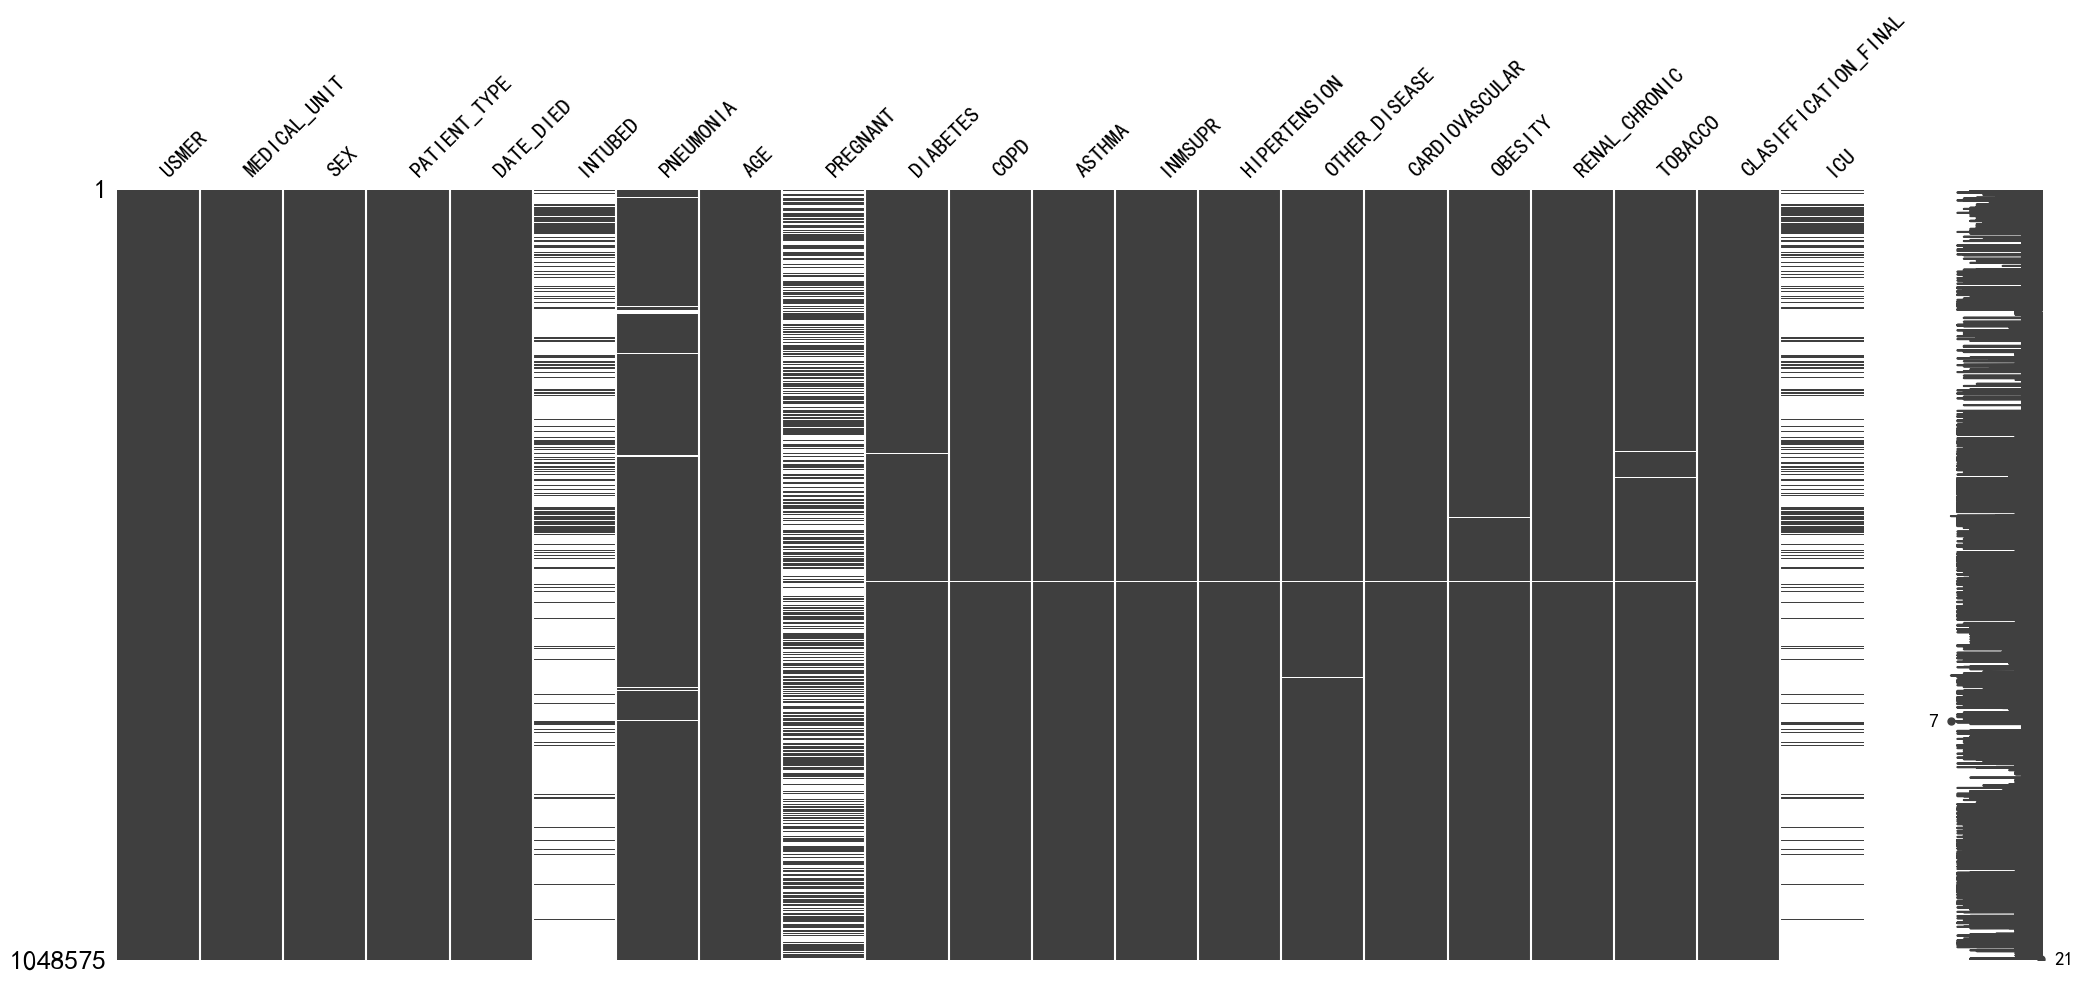
\includegraphics[width=\linewidth]{pic/missing_value.png}
    \caption{Missing value visualization}
    \label{missing_value}
\end{figure}

The methods and reasons for handling missing values are as follows:

\begin{enumerate}
    \item Delete variables with a large number of missing values —— \textbf{icu} and \textbf{intubed}, the reasons are as follows:
    
    A high proportion of missing values may indicate serious issues with the data quality of this variable. The large number of missing values may lead to inaccurate or biased analysis results, thereby reducing the reliability of the data. What's more ,a high proportion of missing values may indicate serious issues with the data quality of this variable. The large number of missing values may lead to inaccurate or biased analysis results, thereby reducing the reliability of the data.
    
    \item Fill in based on other variable information —— \textbf{pregnant}, the methods are as follows:
    
    Due to the inability of men to conceive, some missing values can be filled in based on gender information, and the pregnancy value of the sample with male gender can be supplemented to 0.

    \item Variables with a small number of remaining missing values are filled using the plurality —— \textbf{pneumonia diabetes copd asthma inmsupr hipertension other disease cardiovascular obesity renal chronic tobacco}, the reasons are as follows:

    Since the number of missing values is relatively small, the use of plural padding allows for a larger amount of data to be retained. Removing samples with missing values may result in a reduced amount of data, thus reducing the number of samples for analysis and modeling. By populating with missing values, more data can be retained and maximum use can be made of the available information.Further more,Using the plural to fill in missing values can help maintain the distribution characteristics of the data. The plurality is the most frequent value in the data set, and filling in the missing values allows the populated data to remain similar to the distribution of the original data. This helps avoid introducing excessive bias or distorting the data distribution during the filling process.

\end{enumerate}

\subsection{Outlier Detection}

This study uses the Isolation Forest model for outlier detection, which is an integrated learning-based algorithm for outlier detection. It is based on the following two assumptions:

1. Few outliers: Outliers account for a relatively small percentage of the data and are easier to isolate compared to normal samples.

2. Outliers are easily isolated: there is a significant difference between the features of outliers and those of normal samples, making it easier to isolate the outlier samples.

Based on the above assumptions, the isolated forest uses a top-down recursive partitioning strategy to isolate the abnormal samples.

The algorithm steps are as follows:

1. Select a random feature and a random cut-off value to partition the dataset into left and right subtrees.
2. Repeat step 1 to recursively partition each subtree until a predefined stopping condition is reached, such as reaching a specified tree depth or having only one sample in the subtree.
3. Construct multiple such subtrees to form an isolated forest.
4. The path length (i.e., the number of edges passed from the root node to the abnormal sample) of the outliers is shorter, while the path length of the normal samples is longer. The anomaly score of the sample can be calculated based on the path length.
5. Based on the anomaly score to determine whether the sample is an outlier or not.

The isolated forest quickly isolates the abnormal samples by constructing a random division, where the abnormal samples have shorter path lengths in the tree, while the normal samples have longer path lengths. This fast isolation process makes isolated forests show high efficiency and accuracy in outlier detection.

It should be noted that isolated forest may not perform well for high-dimensional data and noisier datasets. In practical applications, it can be combined with other methods for comprehensive outlier detection.

\subsection{Descriptive Analysis}

After data cleaning, the results of descriptive analysis of the data are as follows (Table \ref{attribute3}):

\begin{table}[hbt!]
    \begin{threeparttable}
    \caption{Descriptive Analysis}
    \label{attribute3}
    \begin{tabular}{llllllll}
        \toprule
        \headrow Feature Name & Mean & Std & Min & 25\% & 50\% & 75\% & Max\\
        \midrule
        sex & 0.500741 & 0.500000 & 0.0 & 0.0 & 1.0	& 1.0 & 1.0\\ 
        \midrule
        age & 41.794102	& 16.907389	& 0.0 & 30.0 & 40.0 & 53.0 & 121.0\\ 
        \midrule
        classification & 5.305653 & 1.881165 & 1.0 & 3.0 & 6.0 & 7.0 & 7.0\\ 
        \midrule
        patient type & 0.809235 & 0.392904 & 0.0 & 1.0 & 1.0 & 1.0 & 1.0\\ 
        \midrule
        pneumonia & 0.135621 & 0.342385 & 0.0 & 0.0 & 0.0 & 0.0 & 1.0\\ 
        \midrule
        pregnancy & 0.007782 & 0.087873 & 0.0 & 0.0 & 0.0 & 0.0 & 1.0\\ 
        \midrule
        diabetes & 0.119580 & 0.324469 & 0.0 & 0.0 & 0.0 & 0.0 & 1.0\\ 
        \midrule
        copd & 0.014406 & 0.119155 & 0.0 & 0.0 & 0.0 & 0.0 & 1.0\\ 
        \midrule
        asthma & 0.030195 & 0.171124 & 0.0 & 0.0 & 0.0 & 0.0 & 1.0\\ 
        \midrule
        inmsupr & 0.013558 & 0.115645 & 0.0 & 0.0 & 0.0 & 0.0 & 1.0\\ 
        \midrule
        hypertension &  0.155651 & 0.362525 & 0.0 & 0.0 & 0.0 & 0.0 & 1.0\\ 
        \midrule
        cardiovascular &  0.019865 & 0.139537 & 0.0 & 0.0 & 0.0 & 0.0 & 1.0\\ 
        \midrule
        renal chronic &  0.018080 & 0.133241 & 0.0 & 0.0 & 0.0 & 0.0 & 1.0\\ 
        \midrule
        other disease & 0.026870 & 0.161704 & 0.0 & 0.0 & 0.0 & 0.0 & 1.0\\ 
        \midrule
        obesity &  0.152855	& 0.359847 & 0.0 & 0.0 & 0.0 & 0.0 & 1.0\\ 
        \midrule
        tobacco &  0.080715	& 0.272397 & 0.0 & 0.0 & 0.0 & 0.0 & 1.0\\ 
        \midrule
        usmr &  0.367806 & 0.482208	& 0.0 & 0.0 & 0.0 & 1.0 & 1.0\\ 
        \midrule
        medical unit & 8.980565 & 3.723278 & 1.0 & 4.0 & 12.0 & 12.0 & 13.0\\ 
        \midrule
        death &  0.073378 & 0.260756 & 0.0 & 0.0 & 0.0 & 0.0 & 1.0\\ 
        \bottomrule 
    \end{tabular}
\end{threeparttable}
\end{table}

Based on this table, you can analyze the central tendency, variability, and range of each feature.

$\bullet$The "sex" feature has a mean of 0.500741, suggesting a roughly equal distribution of the two categories. The standard deviation of 0.500000 indicates that there is some variation in this feature.

$\bullet$The "age" feature has a mean of 41.794102 and a standard deviation of 16.907389. The minimum age is 0.0, the maximum is 121.0, and the data spans a range of values. The quartiles indicate that 25\% of the ages fall below 30.0, 50\% fall below 40.0, and 75\% fall below 53.0.

$\bullet$The "classification" feature has a mean of 5.305653 and a standard deviation of 1.881165. The values range from 1.0 to 7.0, indicating a categorical variable with several distinct classes.

$\bullet$The "death" feature has a mean of 0.073378, suggesting a relatively low overall mortality rate. The standard deviation of 0.260756 indicates some variation in the death rates across the dataset.

\subsection{Exploratory Analysis}

We perform a detailed visual exploration of the data to analyze the relationships between variables and provide insights for the processing of machine learning algorithm features.

\subsubsection{Correlation Analysis}

\begin{figure}[t]
    \centering
    \includegraphics[width=0.8\linewidth]{pic/Correlation Between Features.png}
    \caption{Correlation Between Features}
    \label{Correlation}
\end{figure}

There is a strong negative correlation between the variable PATIENT TYPE and DEATH, a strong positive correlation between PNEUMONIA and DEATH, and a weak correlation between the remaining variables and DEATH (Figure\ref{Correlation}); we can observe an interesting phenomenon that PNEUMONIA has a strong negative correlation with PATIENT TYPE, meaning that most of the patients who went home did not have symptoms of pneumonia and could be treated for both variables.

Through correlation analysis, it can be found that our predictive variable - DEATH (i.e. whether the patient is at high risk, and if it is Death, it indicates a very serious condition) has a strong negative correlation with the type of care the patient receives. That is, if the patient is already hospitalized, the likelihood of death is high, while if the patient returns home to recuperate on their own, the probability of death is low. The reason for this may be that hospitalization already represents a relatively severe condition, resulting in a higher mortality rate.

Meanwhile, the predictive variable - DEATH has a strong positive correlation with pneumonia, indicating that pneumonia is more likely to lead to death, which is also expected. The predictive variable - DEATH has a weak positive correlation with AGE age. The older the age, the weaker the body generally, and therefore the higher the probability of death. The correlation coefficients of other variables are relatively small, and their predictive effect on the dependent variable may be weak.

\subsubsection{Univariate Analysis}

1.Exploring the AGE distribution

\begin{figure}[!hbtp]
    \centering
    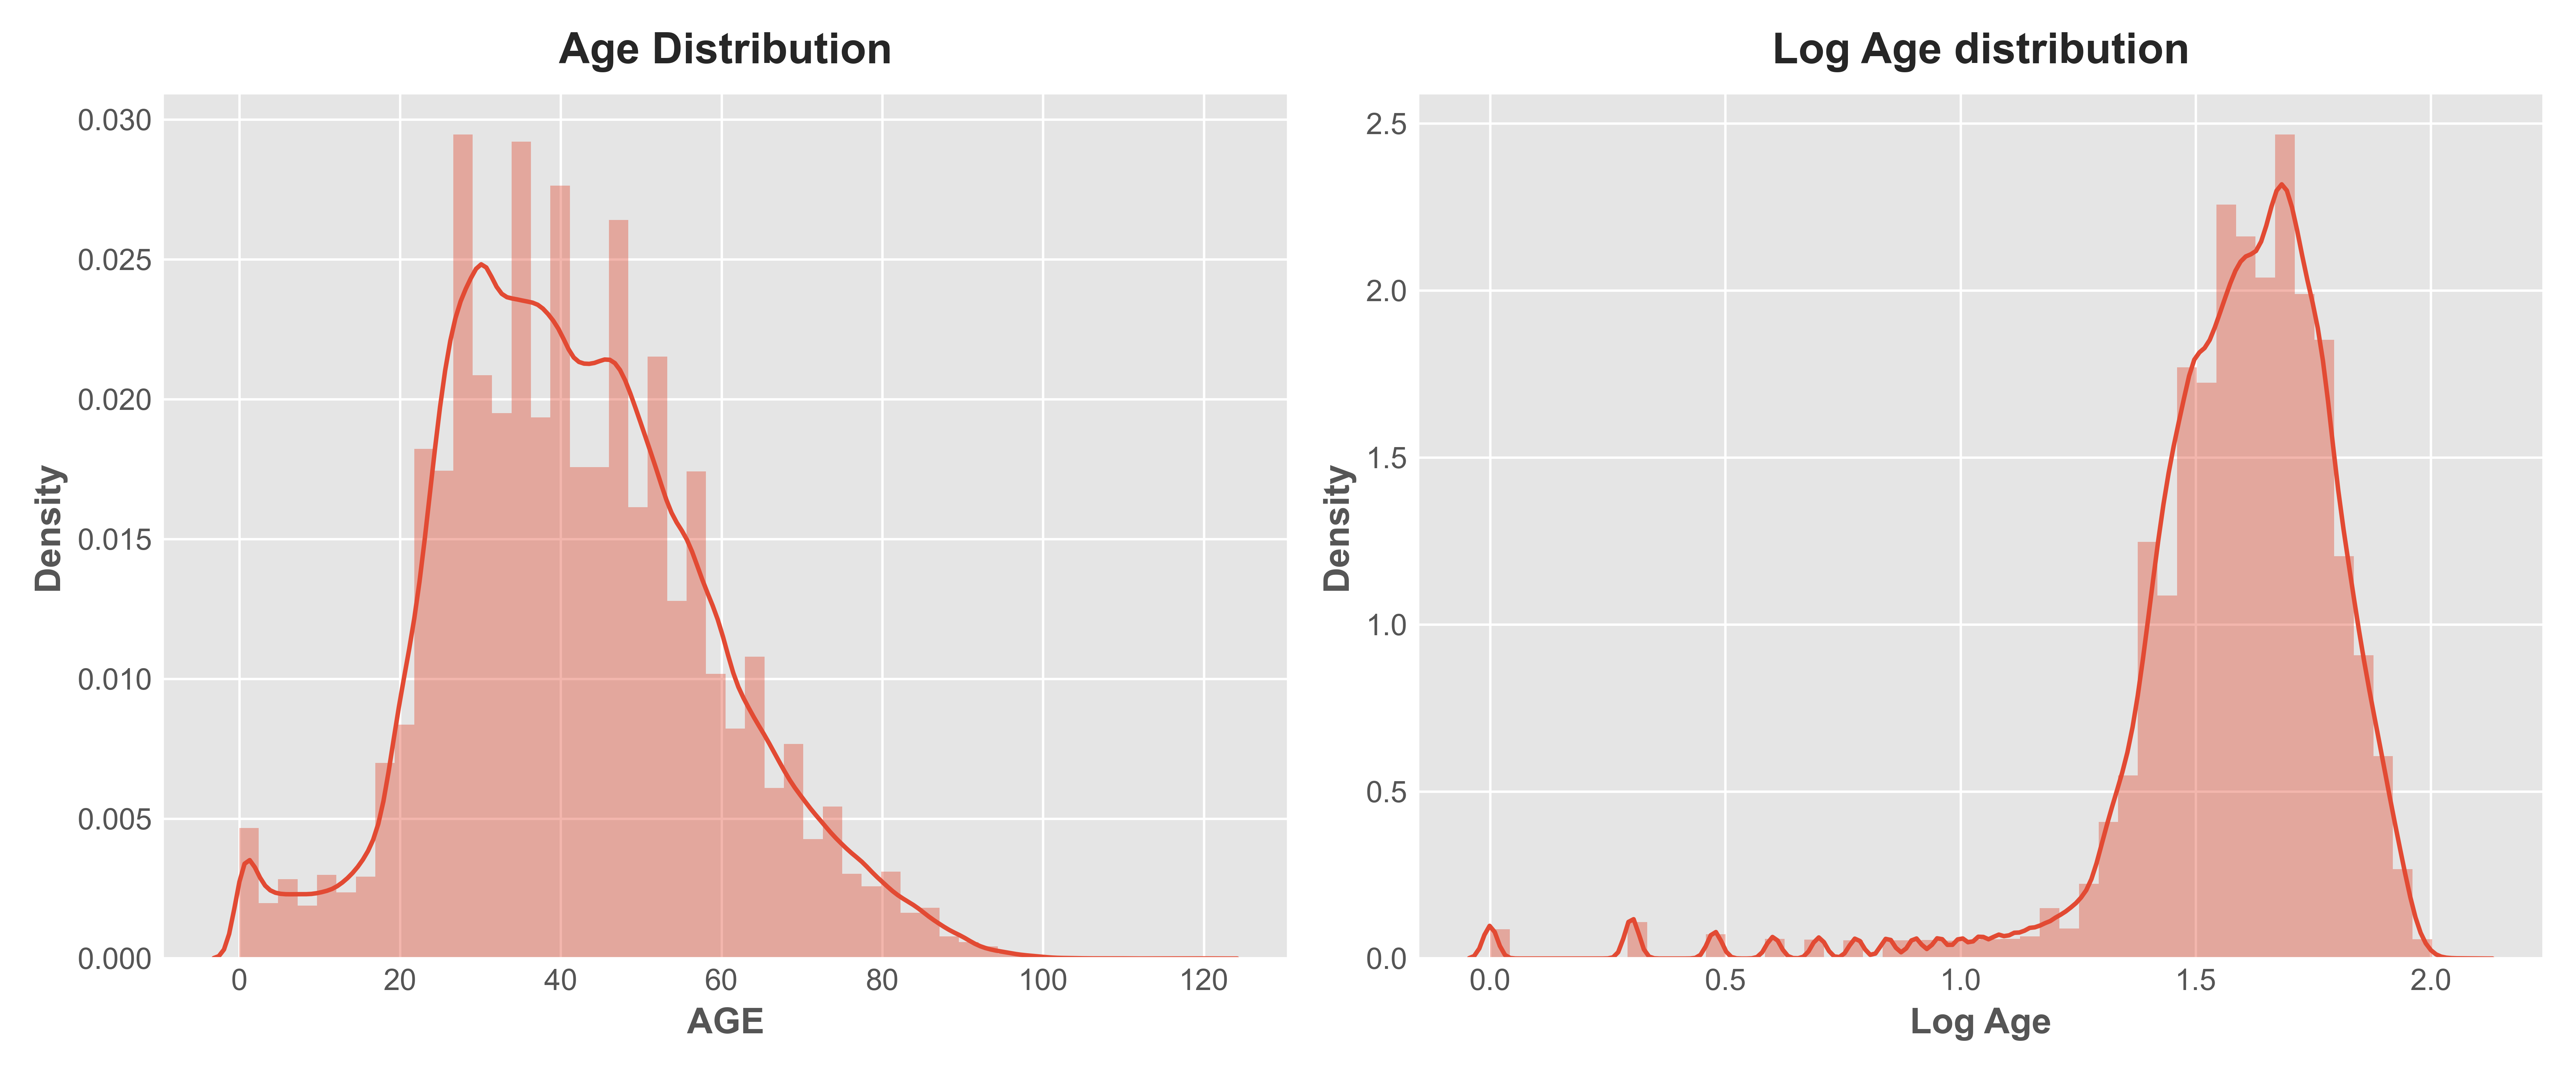
\includegraphics[width=0.9\linewidth]{pic/Age Distribution.png}
    \caption{Age Distribution}
    \label{Age Distribution}
\end{figure}

The age distribution (Figure\ref{Age Distribution}) is approximately normal with a slightly right-skewed distribution. It can be seen that the majority of the survey population is born infants or middle-aged. By log-log processing, we were able to eliminate a small number of outliers at lower ages.

\subsubsection{Multivariate Analysis}

1.The Relationship between AGE and DEATH

\begin{figure}[htbp]
    \centering
    \subfigure[DEATH and AGE HIST RELATION]{
        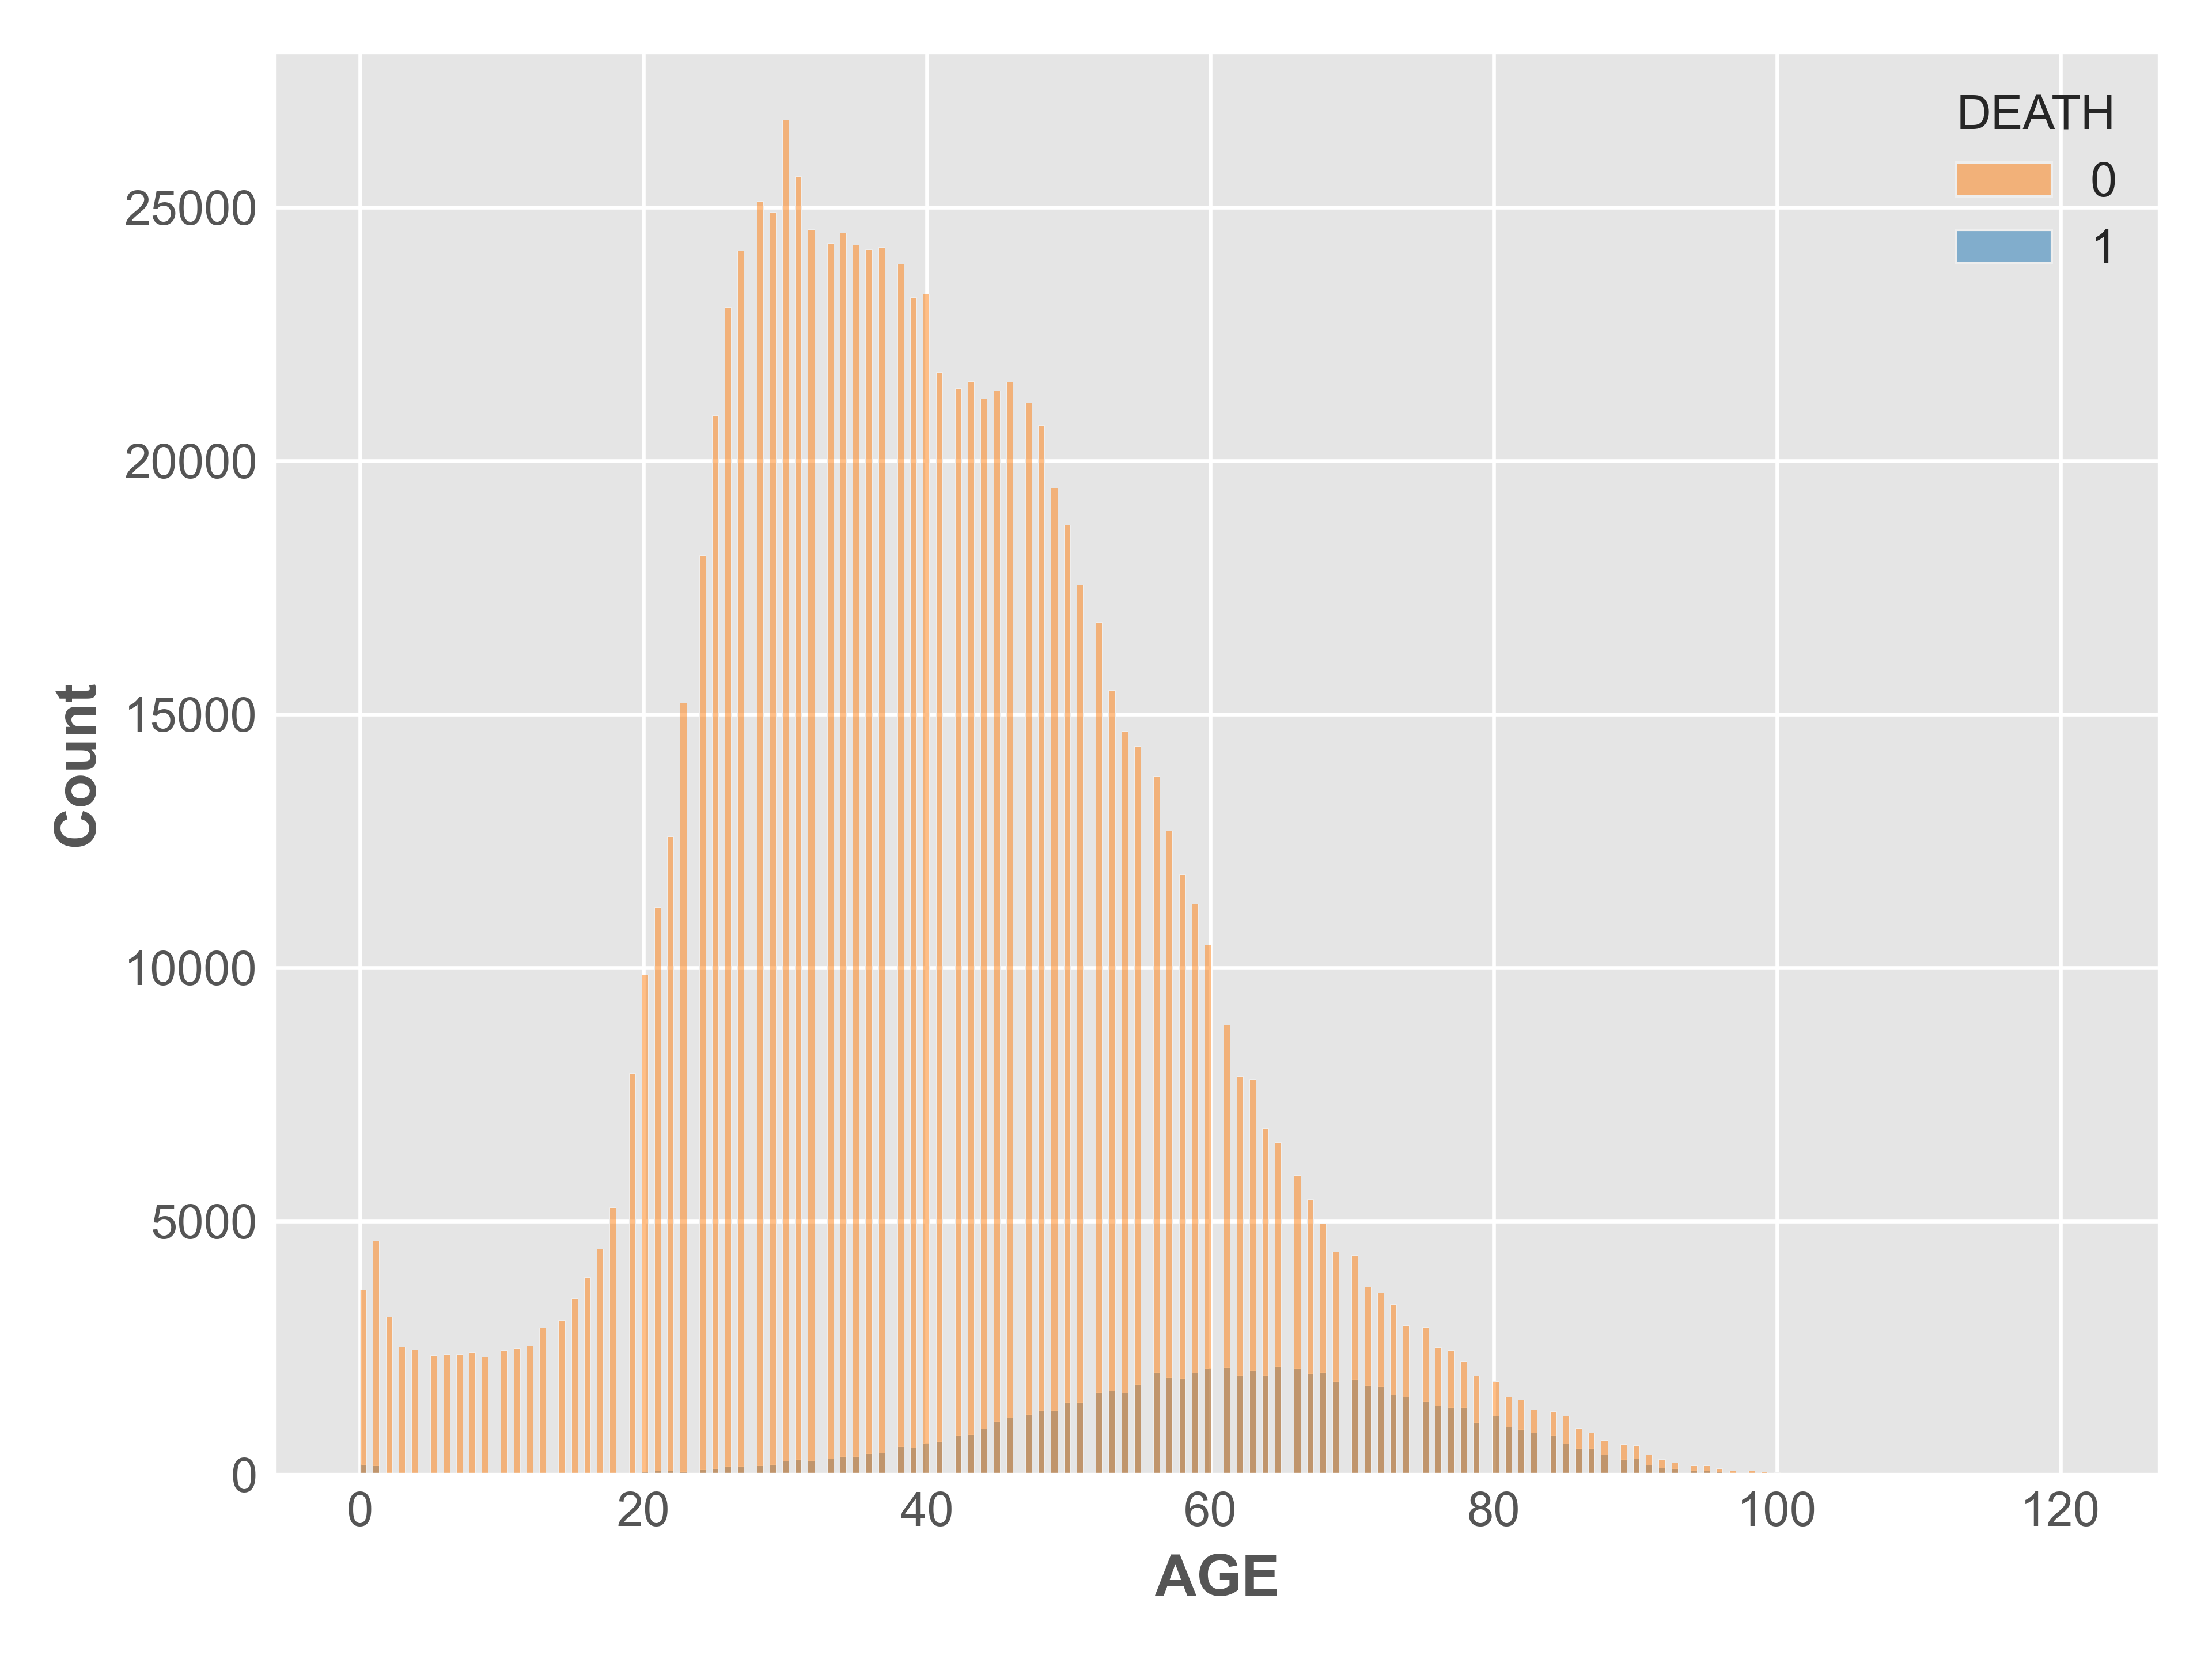
\includegraphics[width=0.49\linewidth]{pic/DEATH_AGE_hist_RELATION.png}
        \label{HIST}
    }
    \hfill
    \subfigure[DEATH and AGE BOX RELATION]{
        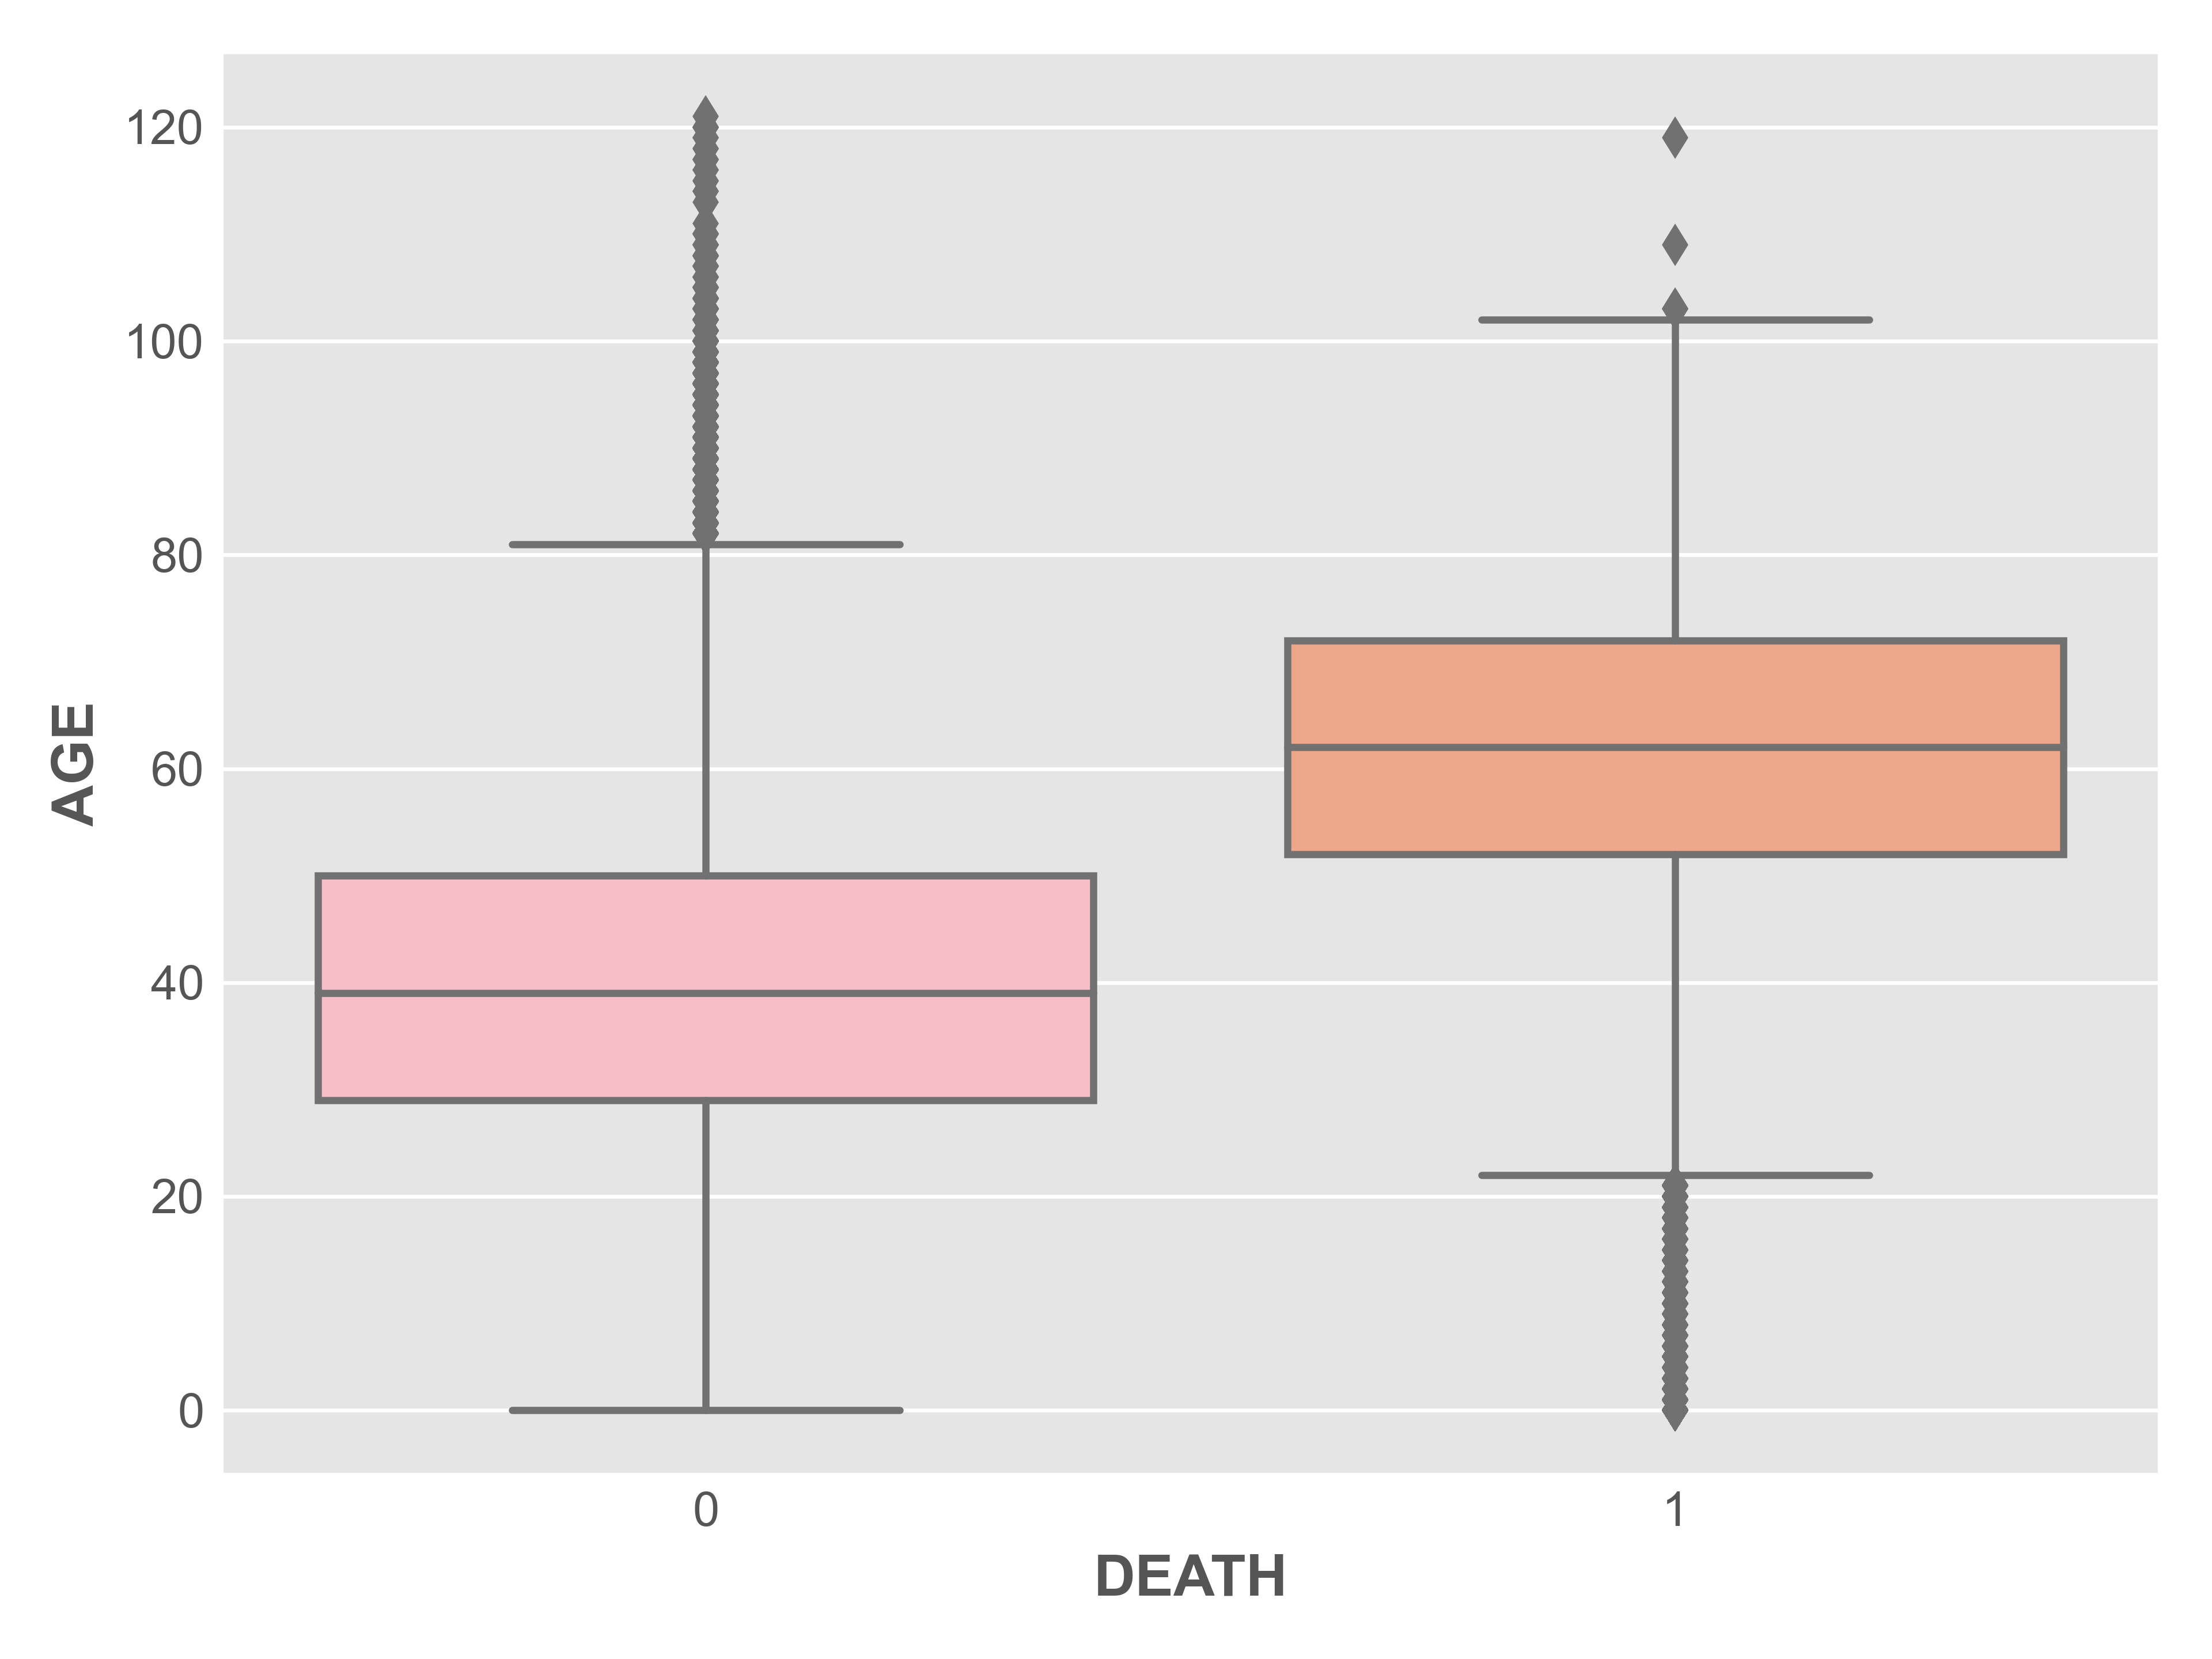
\includegraphics[width=0.49\linewidth]{pic/DEATH_AGE_RELATION.png}
        \label{BOX}
    }
    \caption{DEATH and AGE RELATION}
    \label{combine1}
\end{figure}

The histograms and box plots (Figure\ref{HIST} and Figure\ref{BOX}) show that the age distribution of cured patients approximates the overall distribution (fewer patients died), while patients who died showed an approximate normal distribution with greater variance.

The mean age of cured patients was approximately 40 years, while the mean age of patients who died was approximately 62 years; indicating that the older the age, the greater the probability of dying from the disease.

\newpage
2.The Relationship between PNEUMONIA and DEATH

\begin{figure}[!hbtp]
    \centering
    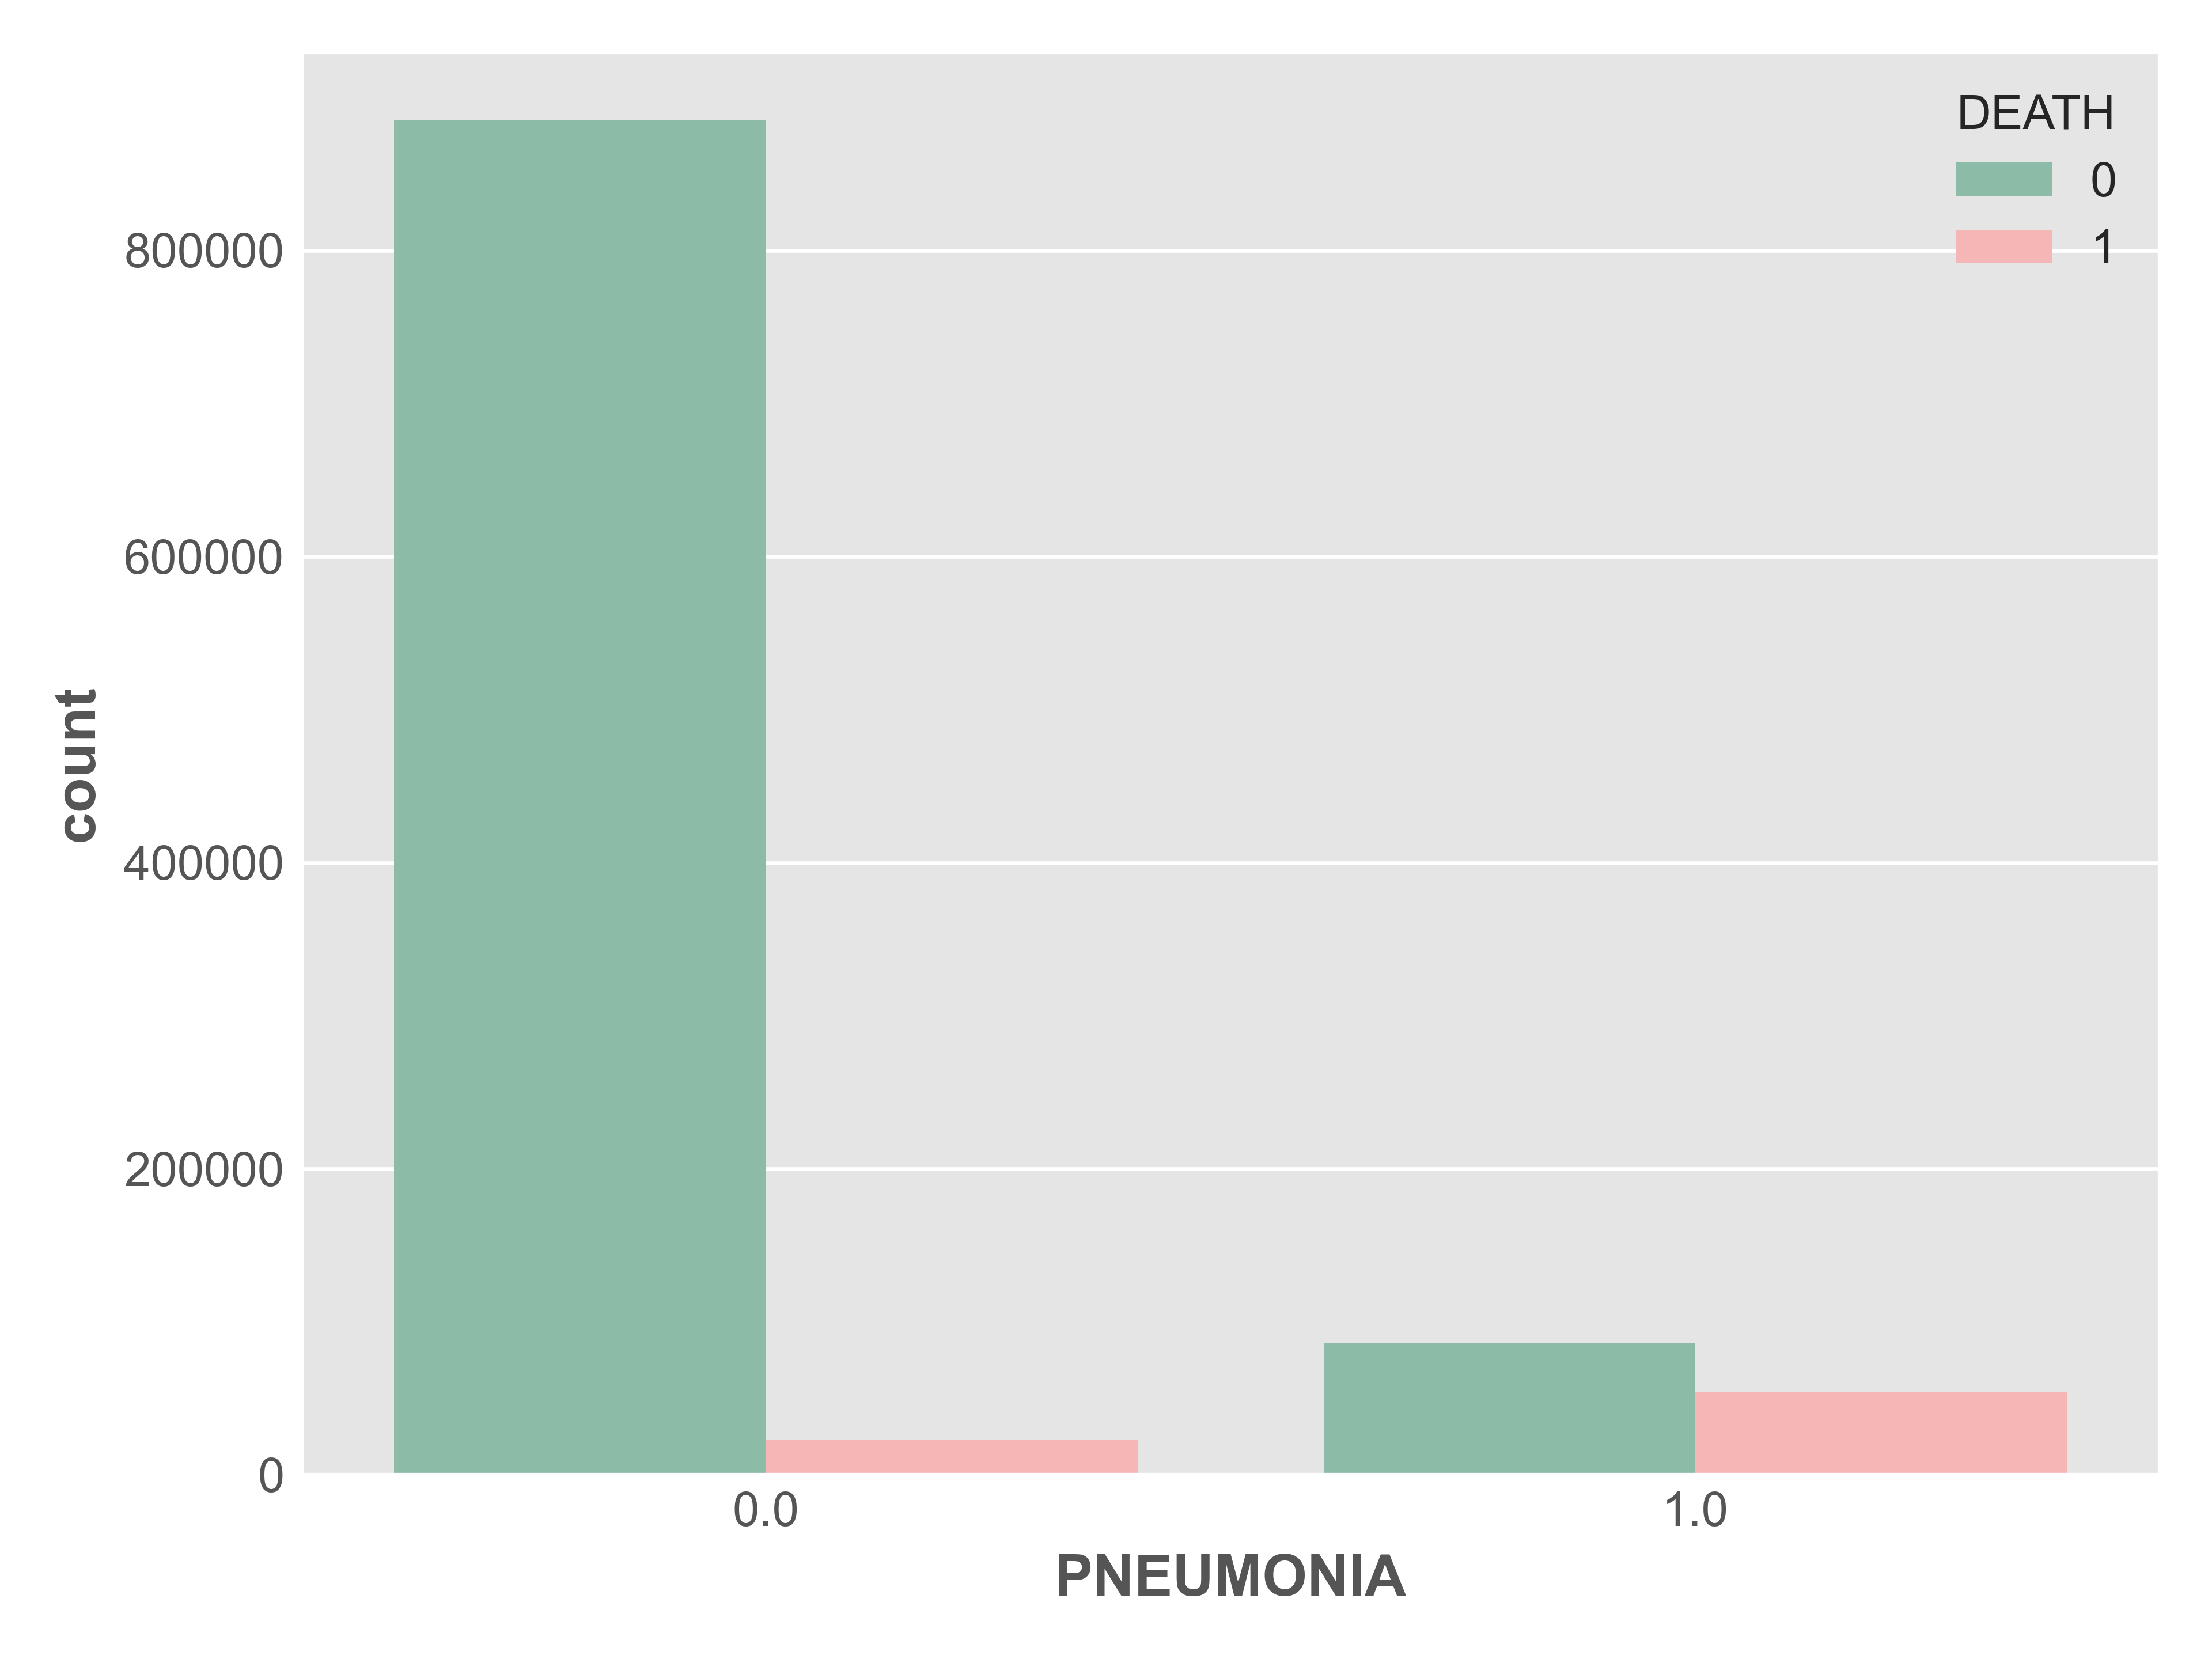
\includegraphics[width=0.6\linewidth]{pic/DEATH_PNEUMONIA_RELATION.png}
    \caption{DEATH and PNEUMONIA RELATION}
    \label{DEATH_PNEUMONIA_RELATION}
\end{figure}

According to the bar chart (Figure\ref{DEATH_PNEUMONIA_RELATION}), we found that the proportion of patients who died after getting pneumonia was significantly higher than that of patients who did not get pneumonia, presumably because one of the key factors in the degree to which COVID-19 become high risk is pneumonia.

3.Relationship between PATIENT TYPE and DEATH

\begin{figure}[!htbp]
    \centering
    \subfigure[DEATH and PATIENT TYPE BAR RELATION]{
        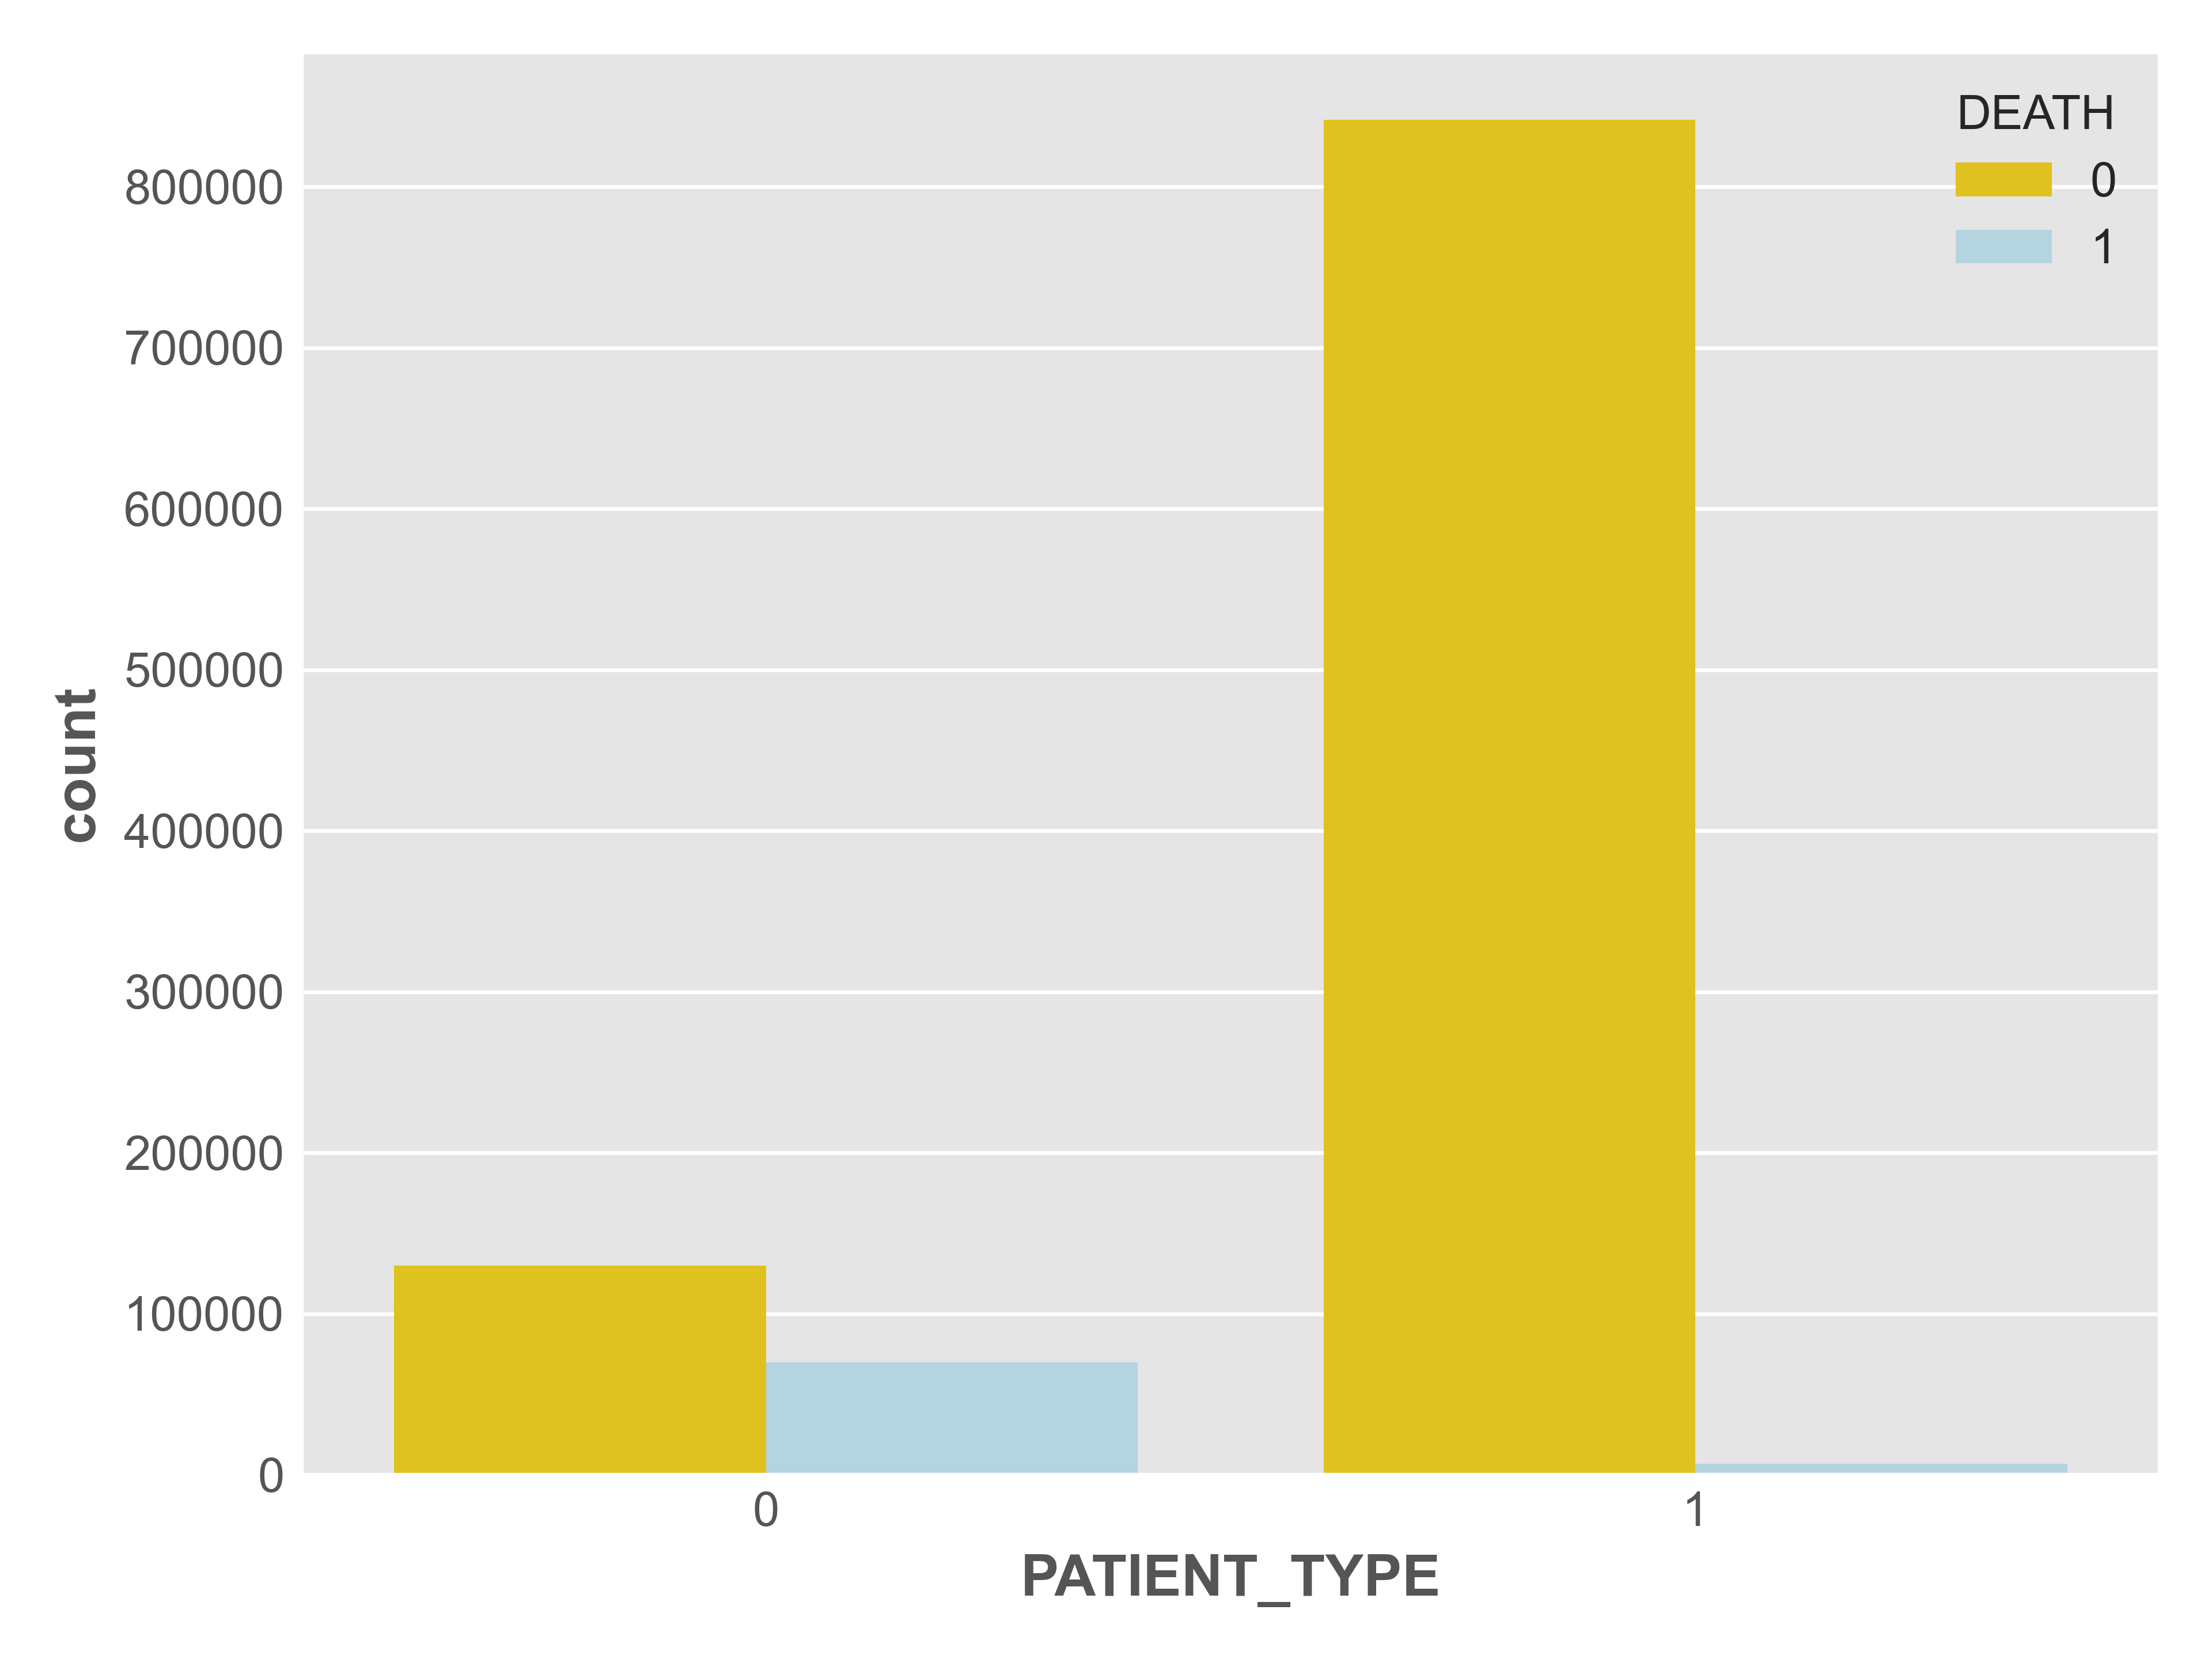
\includegraphics[width=0.49\linewidth]{pic/DEATH_PATIENT_TYPE_RELATION.png}
        \label{DEATH_PATIENT_TYPE_RELATION}
    }
    \hfill
    \subfigure[DEATH and PATIENT TYPE PIE RELATION]{
        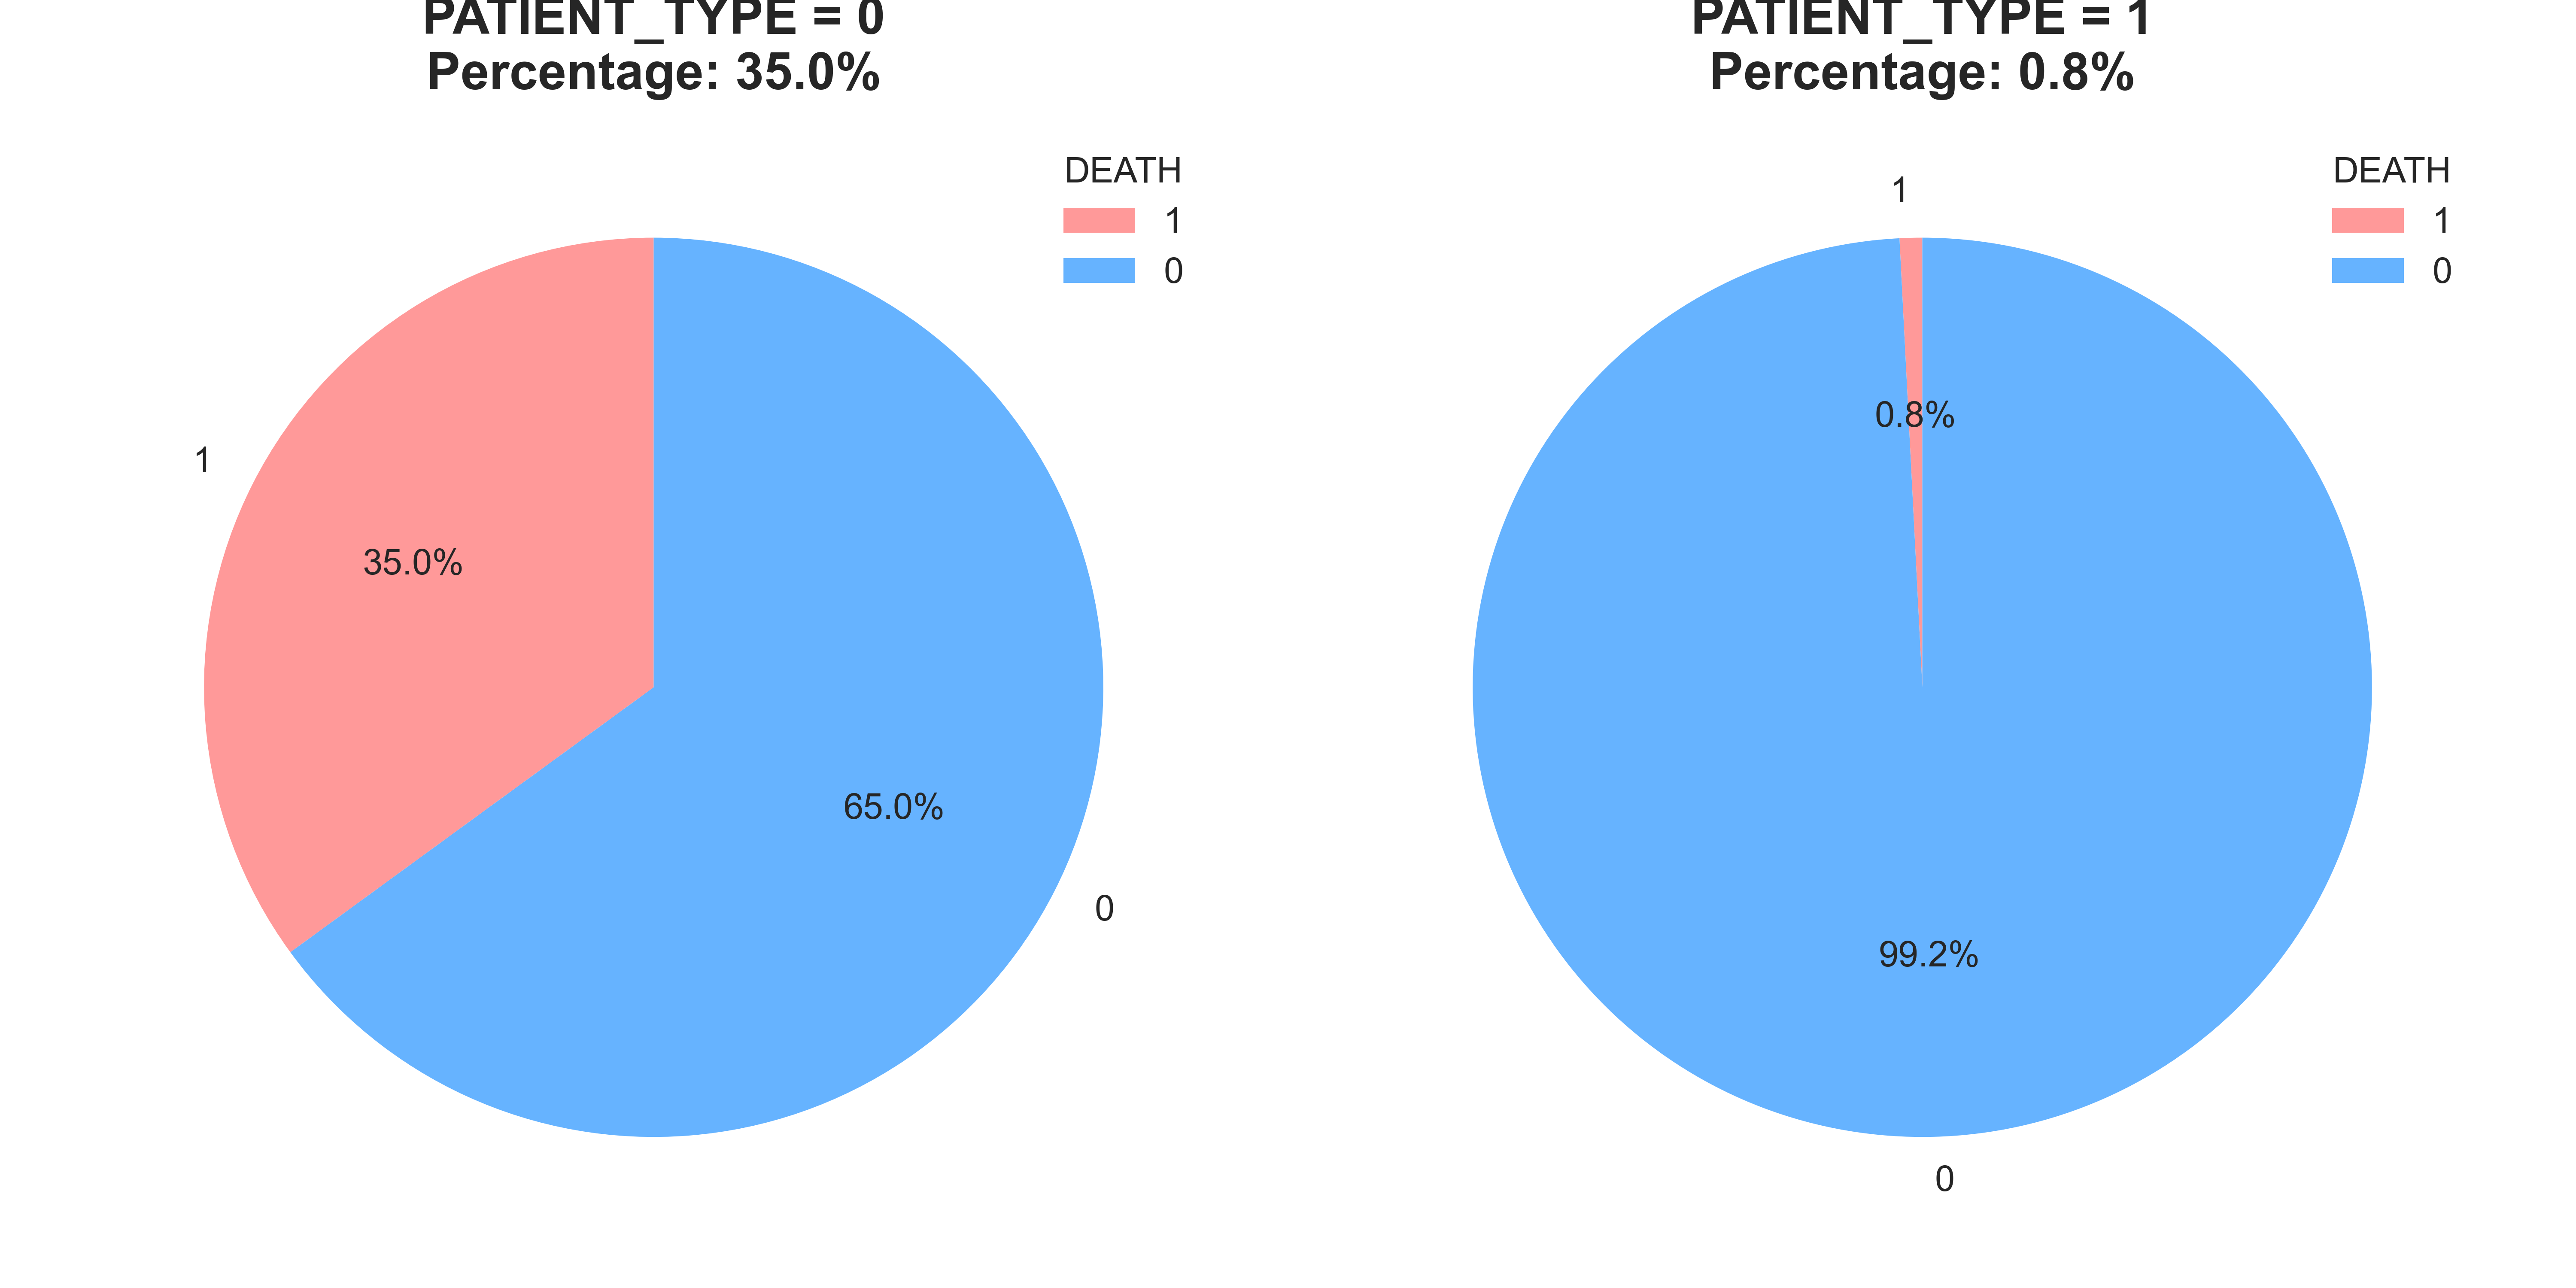
\includegraphics[width=0.49\linewidth]{pic/DEATH_PATIENT_TYPE_PIE_RELATION.png}
        \label{DEATH_PATIENT_TYPE_PIE_RELATION}
    }
    \caption{DEATH and PATIENT TYPE RELATION}
    \label{combine2}
\end{figure}

According to the bar chart and pie chart (Figure\ref{DEATH_PATIENT_TYPE_RELATION} and Figure\ref{DEATH_PATIENT_TYPE_PIE_RELATION}), the probability of death for patients at home is only 0.8\%, compared to a high 35\% probability of death in the hospital. In fact, the relationship between the two is ambiguous, because generally being in hospital care represents that their symptoms are already relatively severe, and even with hospital care, it is not possible to reverse their terminal illness (there are no specific drugs in the early stages of neocoronary, relying mainly on their own immune system). Both can be considered as the same dependent variable, both characterizing whether the patient is already at high risk.

4.Medical Unit, AGE in relation to DEATH

\begin{figure}[!hbtp]
    \centering
    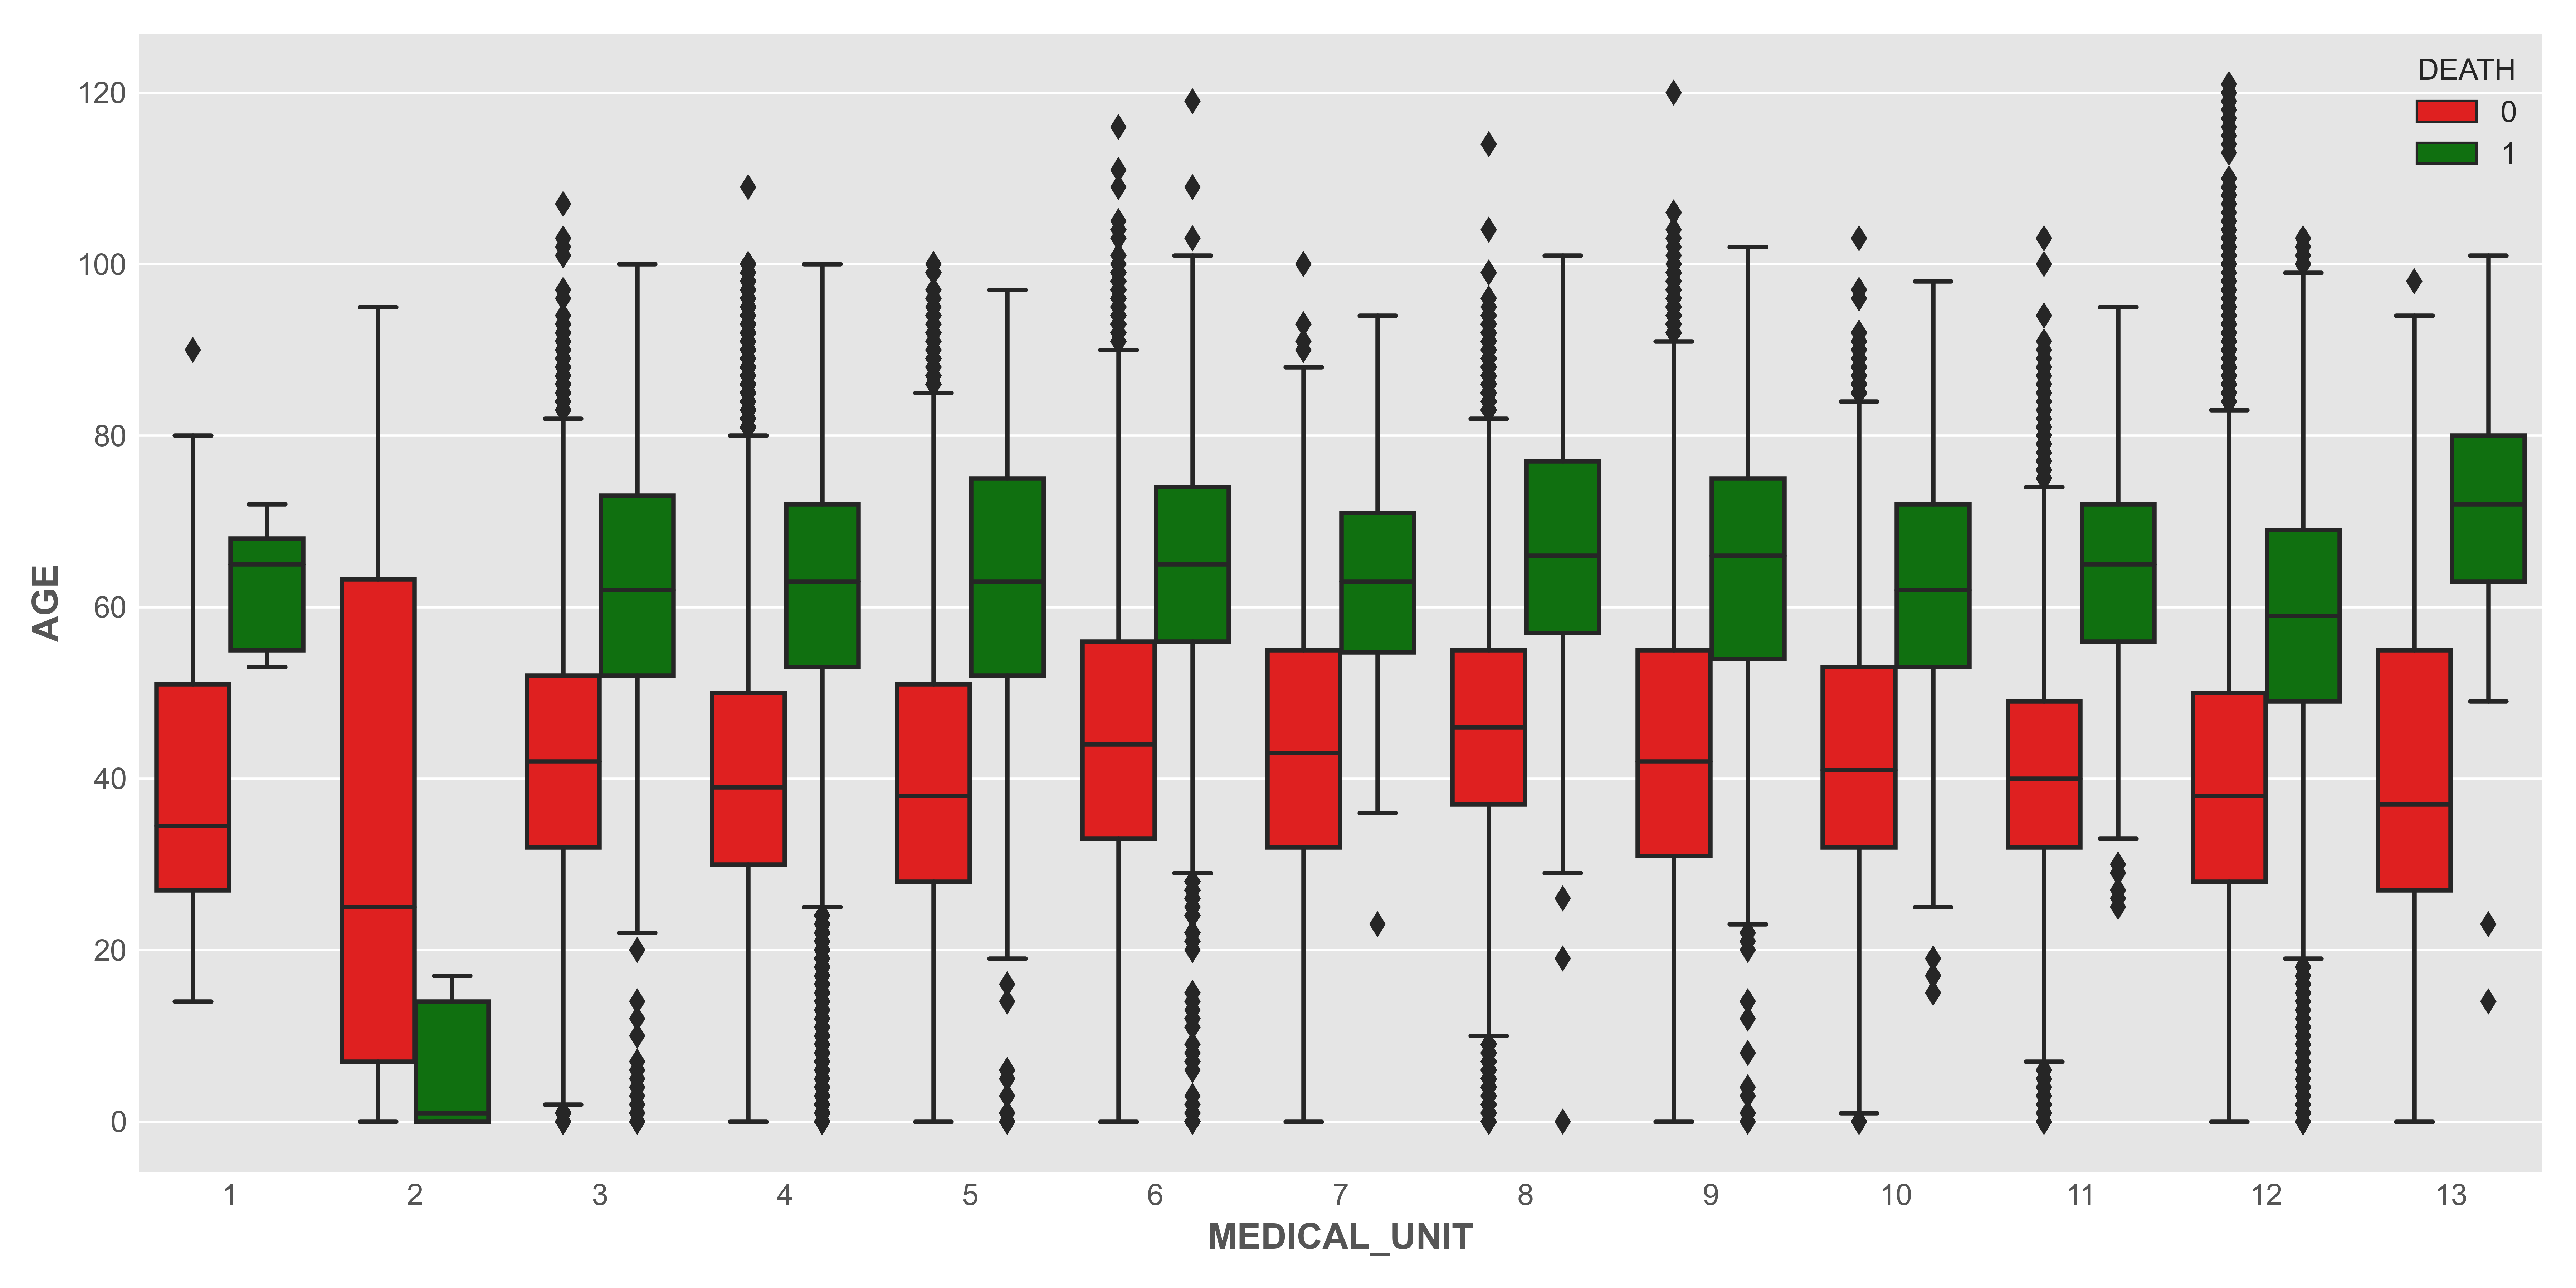
\includegraphics[width=0.9\linewidth]{pic/Distribution of patients who went to medical units by age.png}
    \caption{Distribution of patients who went to medical units by age}
    \label{Distribution of patients who went to medical units by age}
\end{figure}

The box plot (Figure\ref{Distribution of patients who went to medical units by age}) shows that overall the average age at death is still higher than the average age at non-death, and at the same time, we can find some anomalies in provider 2, where the average age at death is lower than the average age at non-death, probably because provider 2 specializes in treating fatal pediatric diseases, which do have a higher mortality rate.

\subsection{Feature Transformation}

\subsubsection{Data normalization}

We standardize the data for the \textbf{AGE} variable for the following reasons:

1. To remove the influence of magnitude: Z-score normalization can remove the influence of magnitude between features. Different features may have different measures (e.g. height, weight, income, etc.), and these different measures may have an impact on some machine learning algorithms. By converting features to the same standard normal distribution, it can make different features comparable and better fit the learning process of the algorithm.

2. Enhance algorithm convergence: Some machine learning algorithms may be more difficult to converge or require longer training time with a larger range of feature values. By scaling the feature values to a smaller range (mean of 0 and standard deviation of 1), Z-score normalization can help the algorithm converge faster.

3. Improve outlier handling: Z-score normalization can effectively handle outliers. Outliers may have a large impact on some machine learning algorithms, making the learning process of the model disturbed. By normalization, outliers will be mapped outside of a larger range of values, thus reducing their impact on the model.

\subsubsection{Dummy variable processing}

Since \textbf{MEDICAL UNIT}, \textbf{CLASIFFICATION FINAL} variables are categorical variables, they are treated as dummy variables.

\subsubsection{Category imbalance processing}

The number of patient survival samples was 971633 and the number of death samples was 76942, which had a serious category imbalance problem, where the number of survival samples was much more than the number of death samples. To solve this problem, we used downsampling to process the data for the following reasons:

1. Our goal is to learn the characteristics of why patients die, so we take downsampling to ensure the accuracy of the death samples.

2. Downsampling may help reduce the risk of noise and overfitting for most classes of samples.

\subsubsection{Handling target leaks}

One problem in this dataset is that the purpose of this question is to predict whether or not the patient is at high risk as a way to save lives. But there is a PATIENT TYPE in the variable, i.e., whether the patient is going home or not. This variable has an information leakage problem: i.e., the training data contains information related to the target variable, but this information is not available in the real application. There is a strong link between being in the hospital or not and whether he is at high risk, usually he is dying already at high risk before he is in the hospital care, and we will not have this information when we actually predict, we are going to see how much medical resources he needs based on his existing status, so we have to delete this variable PATIENT TYPE when we predict.

\section{Algorithm Introduction}

\subsection{Logistic Regression}

Logistic regression is a linear classification model that optimizes parameters by maximum likelihood estimation.

1.Hypothesis space: Logistic regression is a linear classification model that assumes that data can be separated into two categories using a linear function. It assumes a probabilistic relationship between the categories and classifies them by applying a logistic function after linear combination of the input features.

2.Optimization strategy: Logistic regression optimizes the model parameters by maximum likelihood estimation. It maximizes the probability that an observed sample belongs to its true class and minimizes the probability of misclassification.

3.Learning algorithms: Logistic regression uses optimization algorithms such as gradient descent to minimize the loss function and find the parameters that make the model fit the data best.

\subsection{Decision Tree}

Decision tree is a classification and regression model based on a tree structure, and the tree is constructed by selecting the best division.

1.Hypothesis space: Decision tree is a non-parametric classification and regression model based on a tree structure. It assumes that the data can be divided by a series of decision rules and forms a tree structure to make predictions.

2.Optimization strategy: Decision tree optimizes the model by selecting the best division. Commonly used segmentation metrics are Gini impurity and information gain, which measure the degree of improvement in data purity after segmentation on a feature.

3.Learning algorithms: The learning algorithms for decision trees include ID3, C4.5 and CART. These algorithms construct a decision tree with minimum impurity by recursively selecting the best partitioning features and partition points.

\subsection{Gradient Boosting Trees}

LightGBM, XGBoost and CatBoost are gradient boosting tree based algorithms that optimize the model by iteratively training the decision tree.

1.Assumption space: Gradient Boosting Trees is an integrated learning method that builds a more powerful predictive model by combining multiple decision trees. It assumes that the data can be fitted by the integration of multiple decision trees.

2.Optimization strategy: Gradient Boosting Tree trains the decision tree iteratively and uses gradient descent to minimize the loss function. At each iteration, it looks at the residuals of the previous round of model predictions as a way to improve the fit of the model.

3.Learning algorithm: The gradient boosting tree uses a forward stepwise algorithm that reduces the loss function by fitting a decision tree at each step. lightGBM, XGBoost and CatBoost are all improvements and optimizations of the gradient boosting tree to improve the training speed and model performance.

\section{Results and Analysis}

\subsection{Algorithm Performance Comparison}

We will compare these five algorithms from five perspectives, namely generalization ability, computational cost, stability, interpretability, and privacy protection(Table \ref{comparsion1}).

1. Generalization ability: Generalization ability is commonly known as the ability of the learned law (function) to predict unknown data. In practice, we usually evaluate the generalization ability of a learning method by testing the error.

2. Computational cost: It can be evaluated in terms of training time, testing time, storage requirements, and communication cost, all of which are rated as the less the better

3. Stability: The stability of the hyperparameters, the stability of the samples, the stability of the algorithm, and the stability of the environment are evaluated, and they are all evaluated in terms of the degree of impact of small changes on the results, i.e., the smaller the sensitivity, the better.

4. Interpretability: The interpretability of the model and the interpretability of the features can be elaborated.

5. Privacy protection: It can be analyzed from four aspects of anonymity, diversity, proximity, and differential privacy.

\begin{table}[hbt!]
    \begin{threeparttable}
    \caption{Algorithm Performance Comparison}
    \label{comparsion1}
    \begin{tabular}{llllll}
        \toprule
        \headrow Algorithm & Logistic regression & Decision tree & LightGBM & XGBoost & CatBoost \\
        \midrule
        Generalizability(Accuracy)  & 0.87890 & 0.87894 & 0.88355 & 0.88332 & 0.88413	\\ 
        \midrule
        Training Time & 1.81443s & 0.67917s & 0.48101s & 4.9087s & 27.16034s\\ 
        \midrule
        Test Time & 0.0069s & 0.0170s & 0.0539s & 0.0399s & 0.0304s	\\ 
        \midrule
        Storage Requirements & Low & Medium & Low & High & High	\\ 
        \midrule
        Hyperparameters Stability & High & Low & Low & Low & Low	\\ 
        \midrule
        Sample Stability & Low & Medium & High & High & High	\\ 
        \midrule
        Algorithm stability & High & High & Medium & Medium & Medium	\\ 
        \midrule
        Explanatory & High & High & Medium & Medium & Medium	\\ 
        \midrule
        Data Privacy Protection & Low & High & Low & Low & High	\\ 
        \bottomrule 
    \end{tabular}
\end{threeparttable}
\end{table}

Considering the above, we believe that decision tree is the optimal evaluation algorithm with high explanatory power, low computational cost of the algorithm, relatively good generalization ability, slightly less stability, and privacy protection not as the main consideration, and we analyze the results of decision tree model training below.

\subsection{Results}

We will show the results of decision tree model training from four aspects.

1.Decision Tree Model Classification Results Report:

\begin{table}[!htbp]
    \begin{threeparttable}
    \caption{Classification Results}
    \label{Result1}
    \begin{tabular}{lllll}
        \toprule
        \headrow Attribute & Precision & Recall & F1-score & Support\\
        \midrule
        0 & 0.90 & 0.86 & 0.88 & 15296 \\ 
        \midrule
        1 & 0.86 & 0.90 & 0.88 & 15481 \\ 
        \midrule
        accuracy &   &   & 0.88 & 30777\\ 
        \midrule
        macro avg & 0.88 & 0.88 & 0.88 & 30777\\ 
        \midrule
        weighted avg & 0.88 & 0.88 & 0.88 & 30777\\  
        \bottomrule 
    \end{tabular}
\end{threeparttable}
\end{table}

2.Decision Tree Model Confusion Matrix and ROC curve:

\begin{figure}[!htbp]
    \centering
    \subfigure[Confusion Matrix]{
        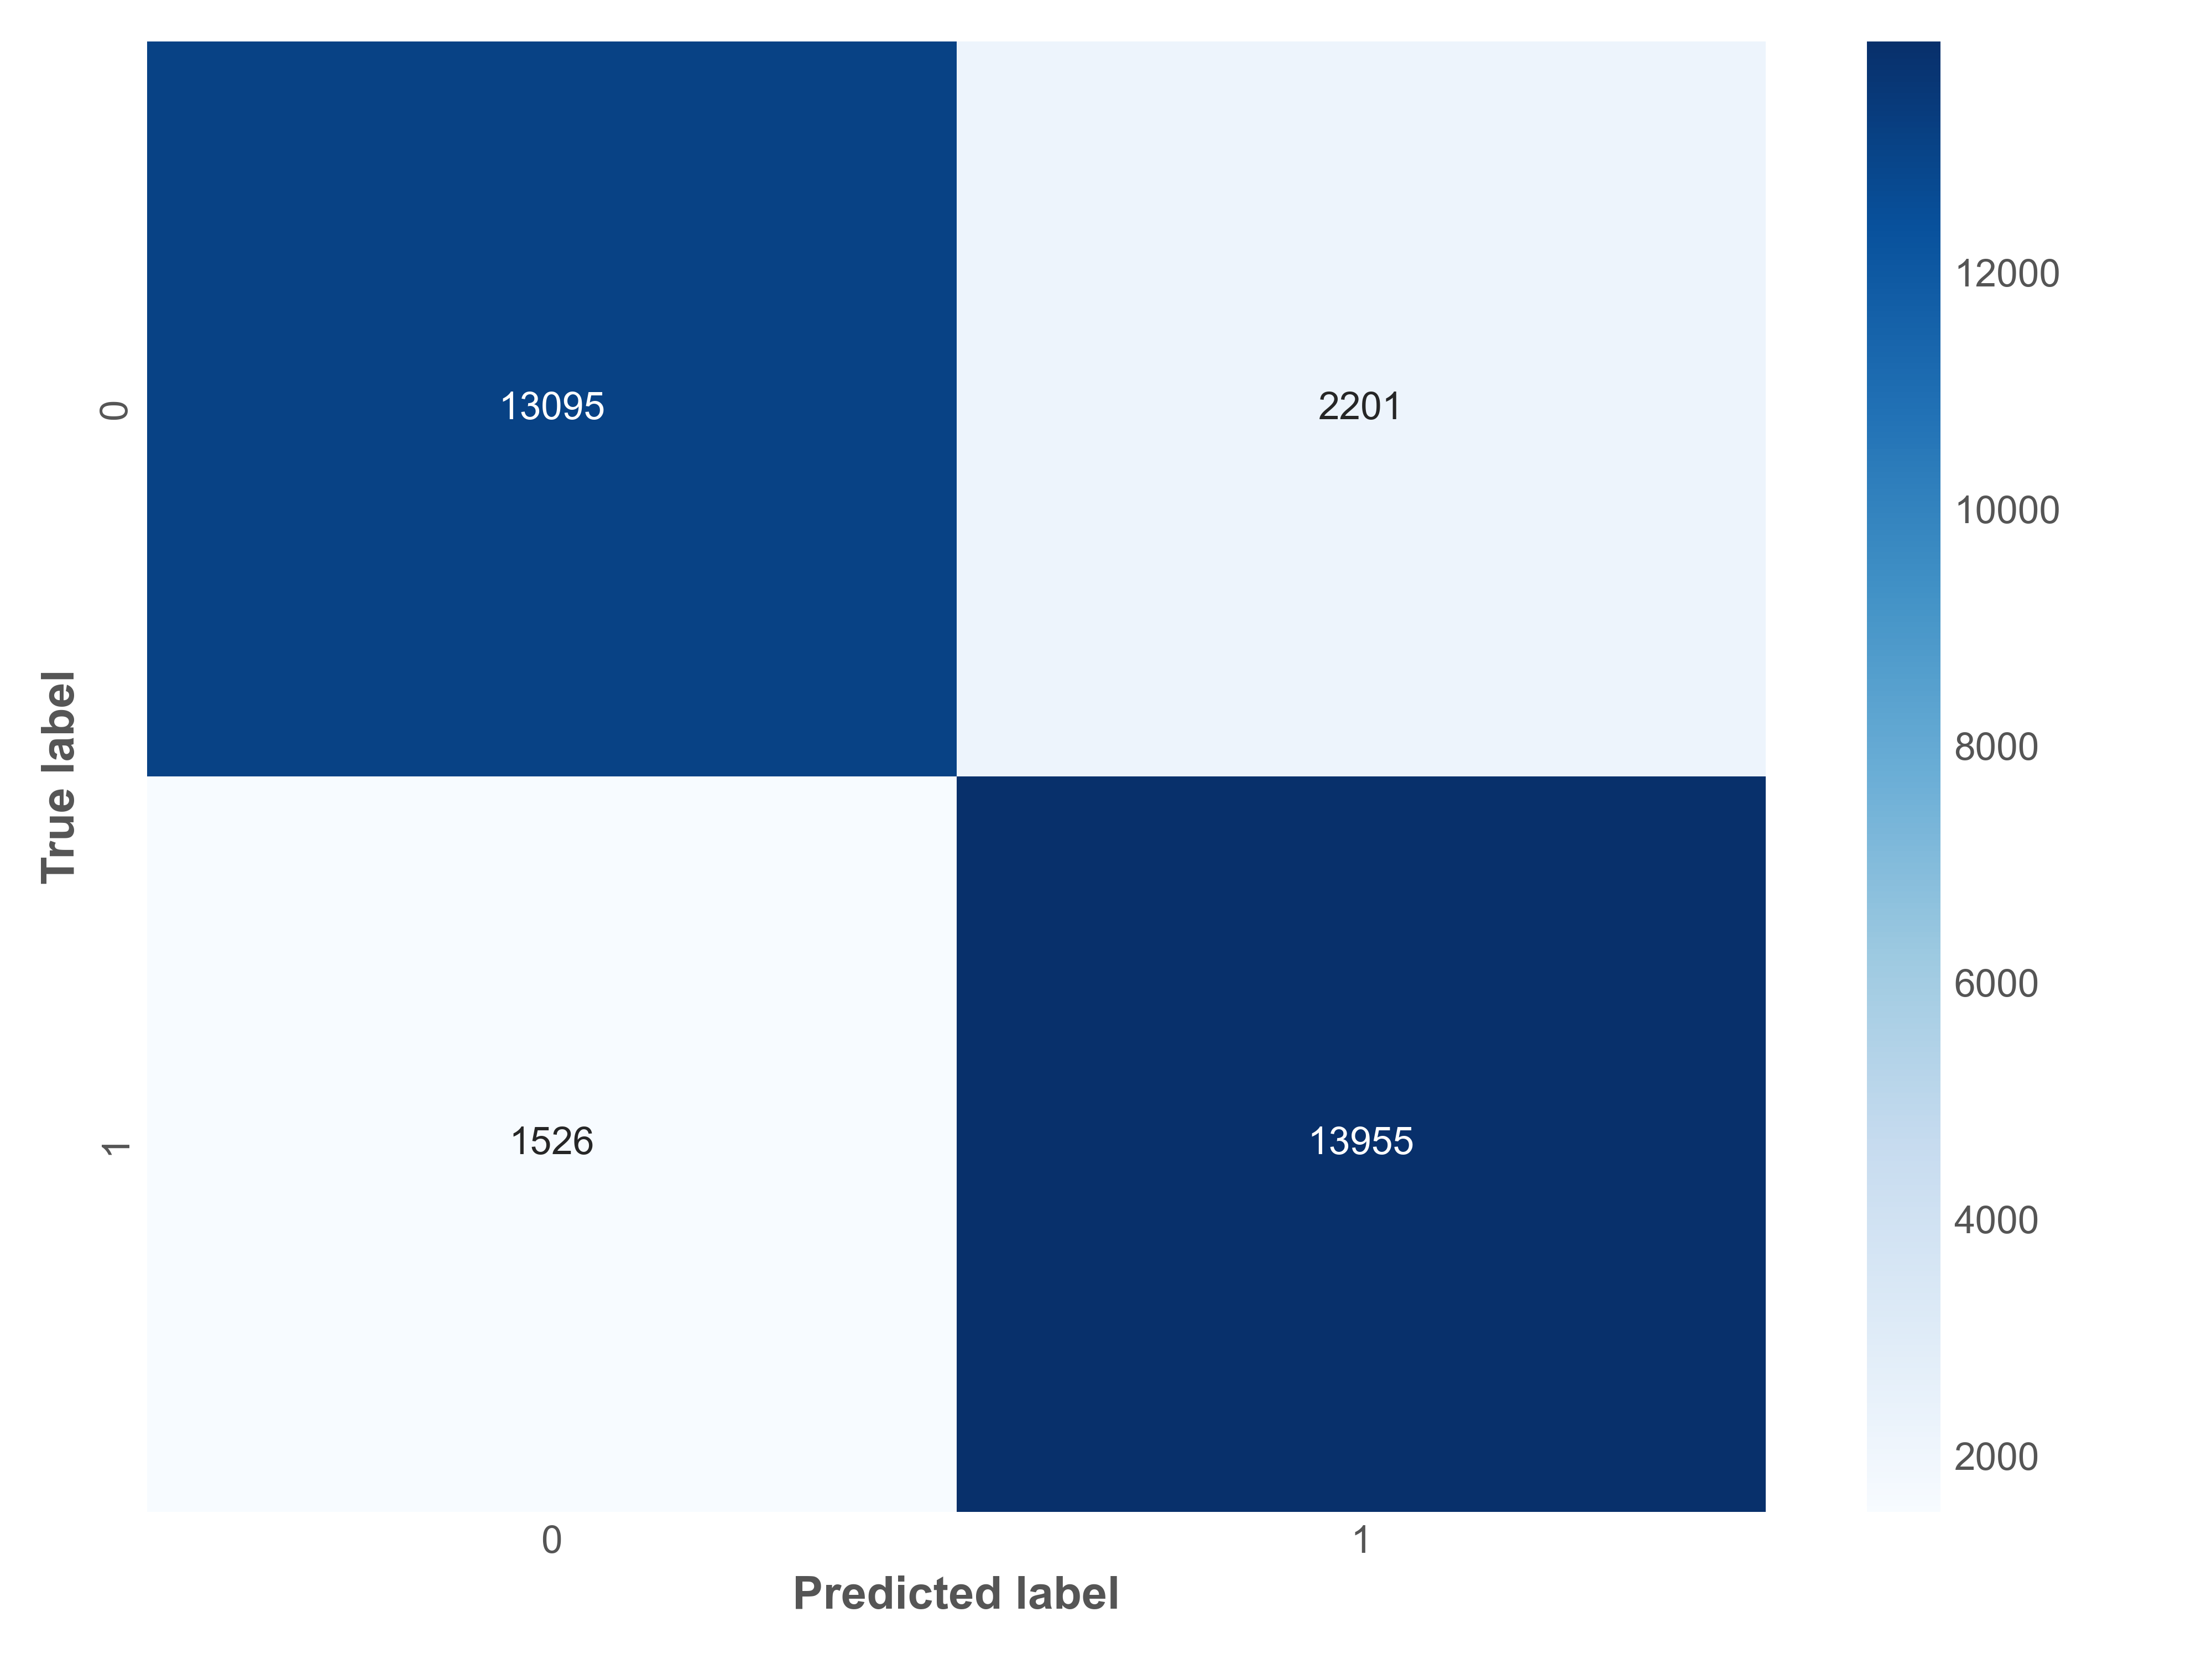
\includegraphics[width=0.49\linewidth]{pic/confusion_matrix.png}
        \label{Confusion Matrix}
    }
    \hfill
    \subfigure[ROC curve]{
        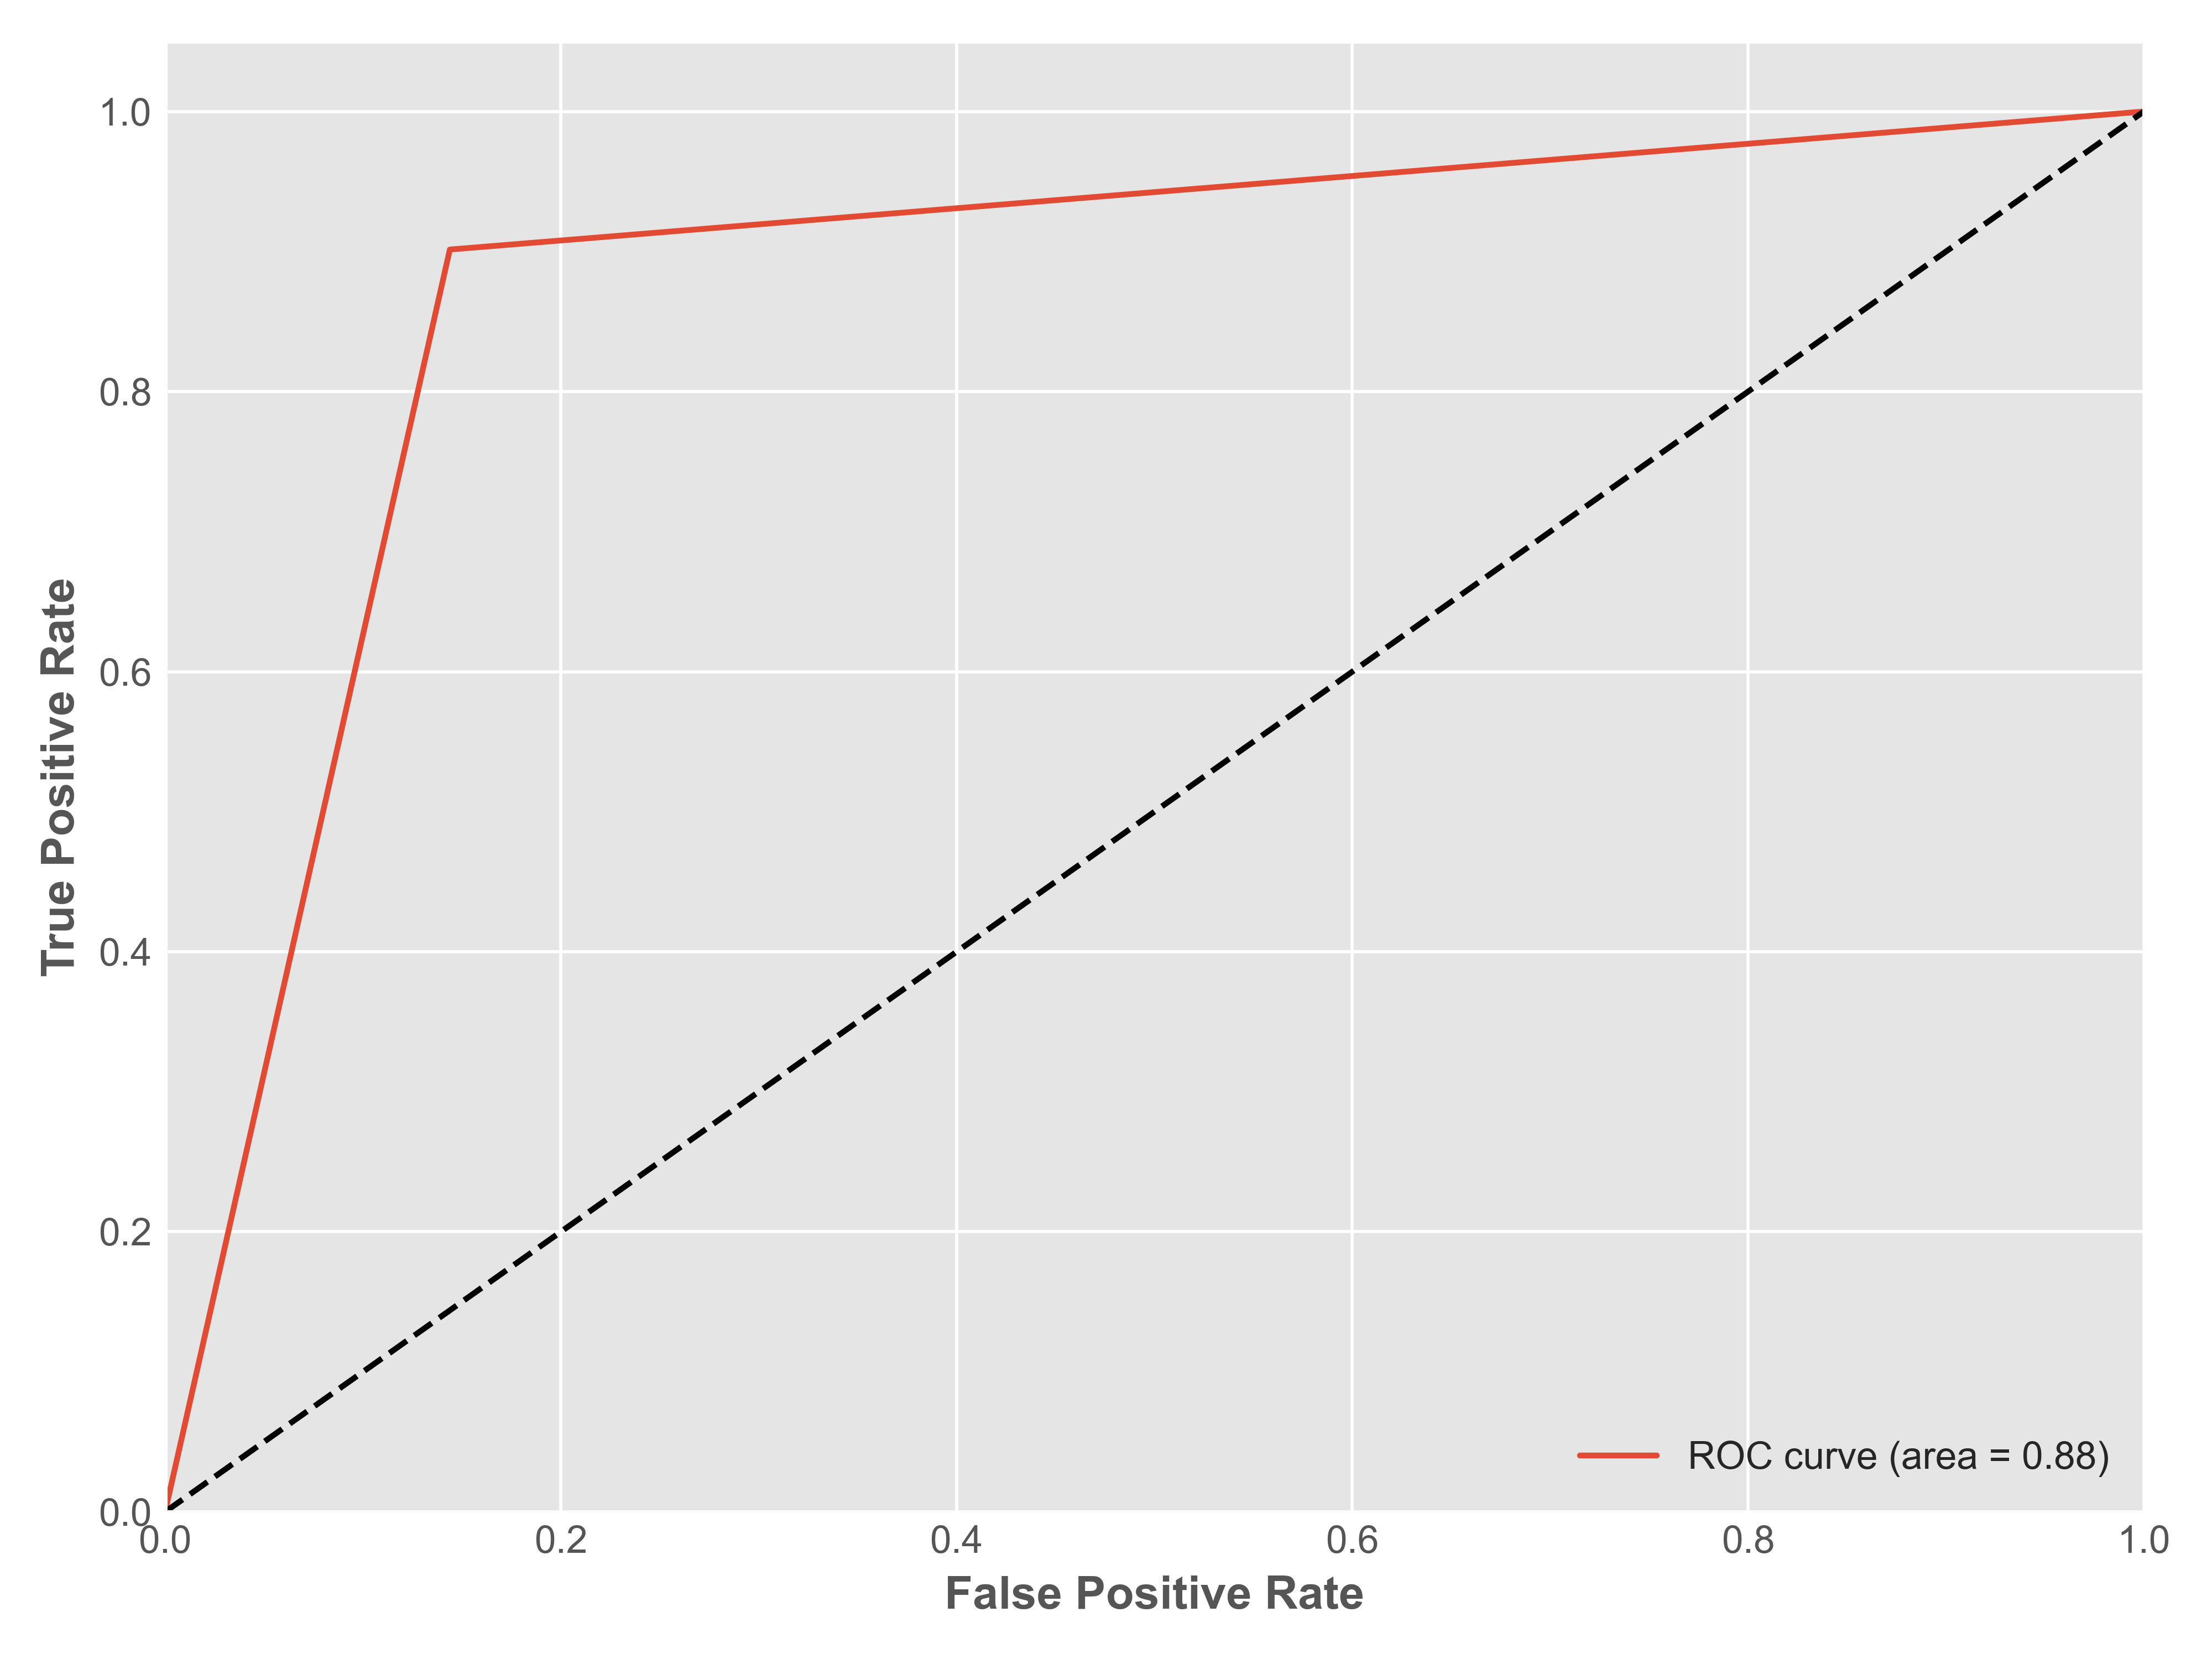
\includegraphics[width=0.49\linewidth]{pic/ROC.png}
        \label{ROC curve}
    }
    \caption{Detail result}
    \label{combine3}
\end{figure}


3.Decision Tree Model Tree Structure Visualization (first three layers):

\begin{figure}[!hbtp]
    \centering
    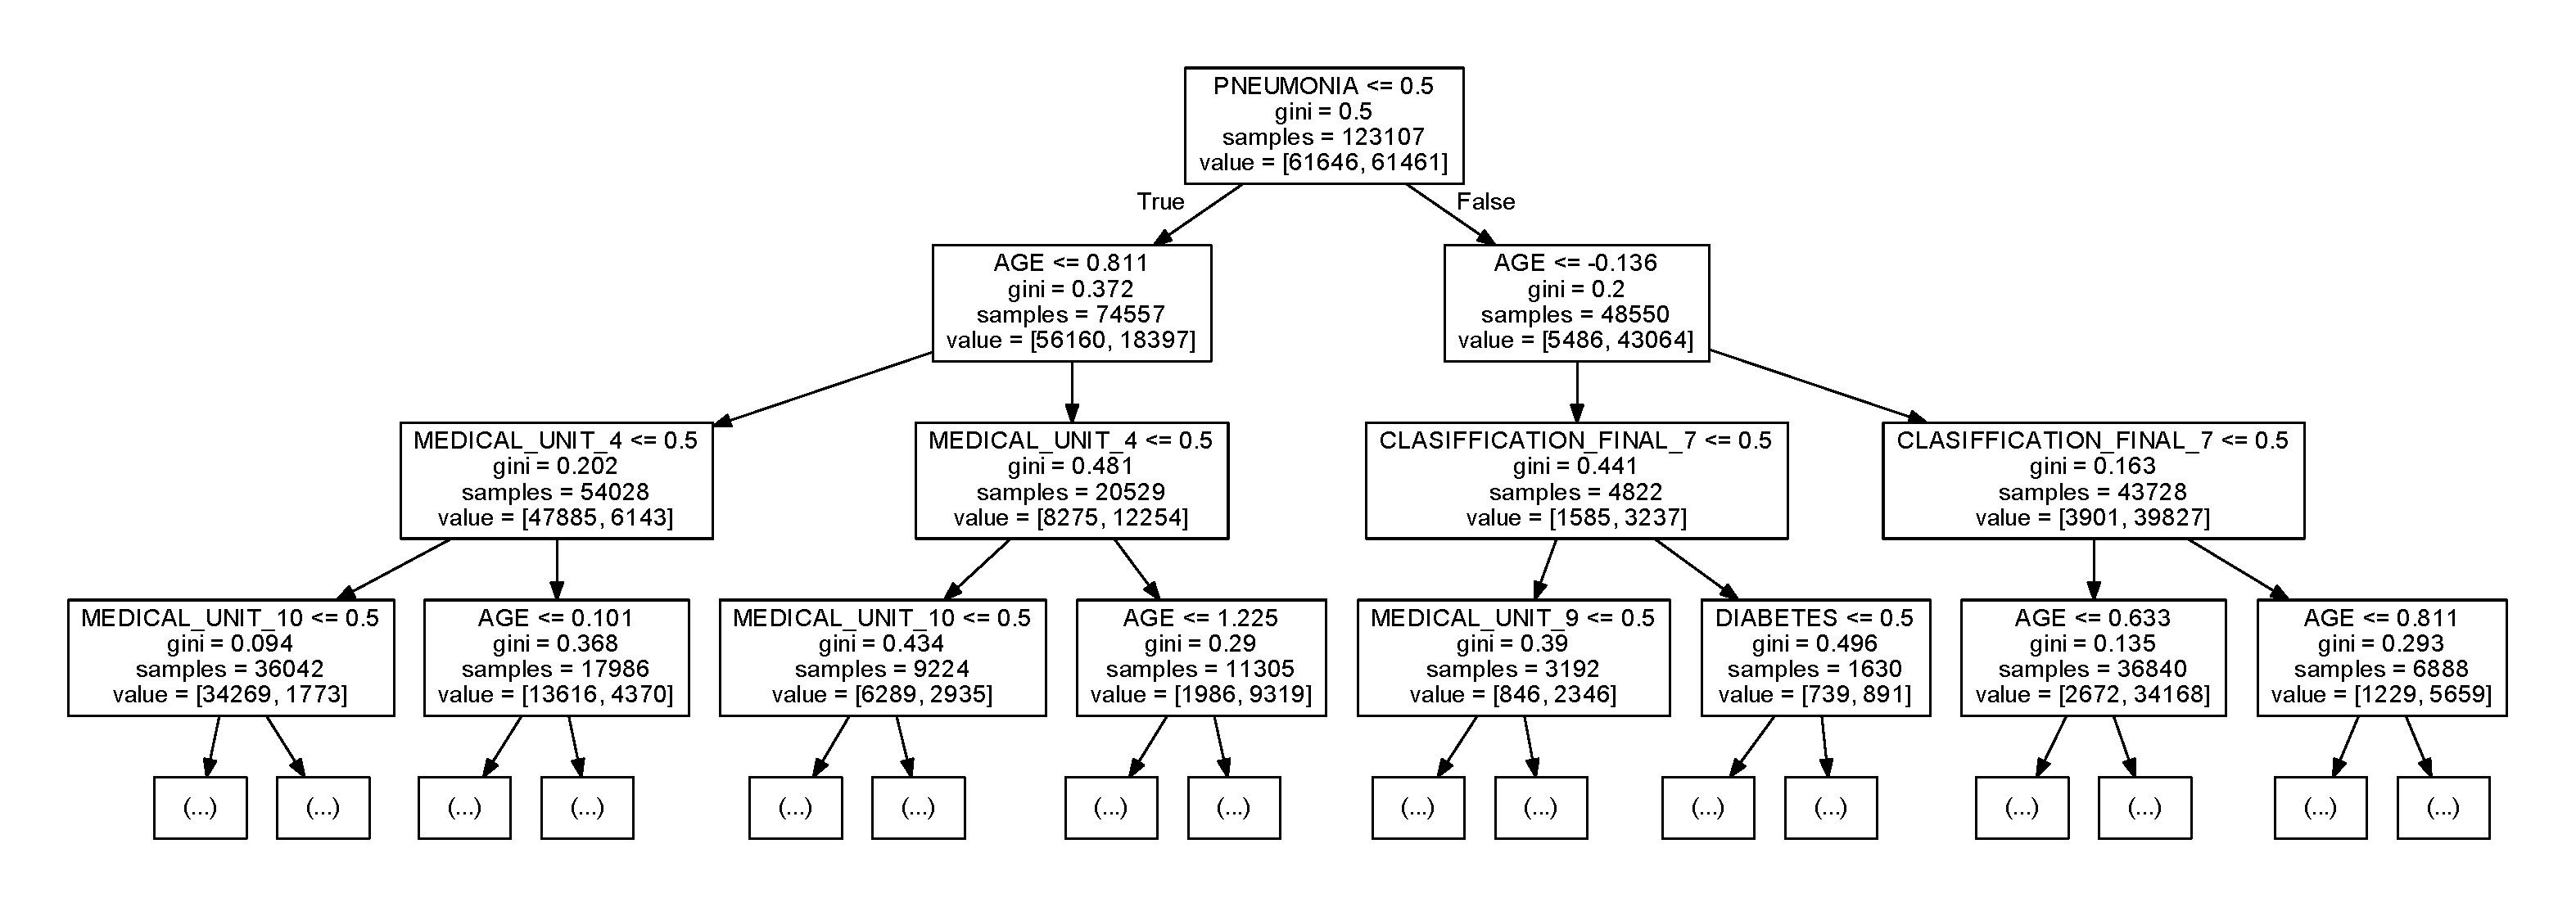
\includegraphics[width=\linewidth]{decision_tree.pdf}
    \caption{Tree Structure Visualization}
    \label{Tree Structure Visualization}
\end{figure}

\newpage
4.Decision Tree Model Feature Importance:

\begin{figure}[!hbtp]
    \centering
    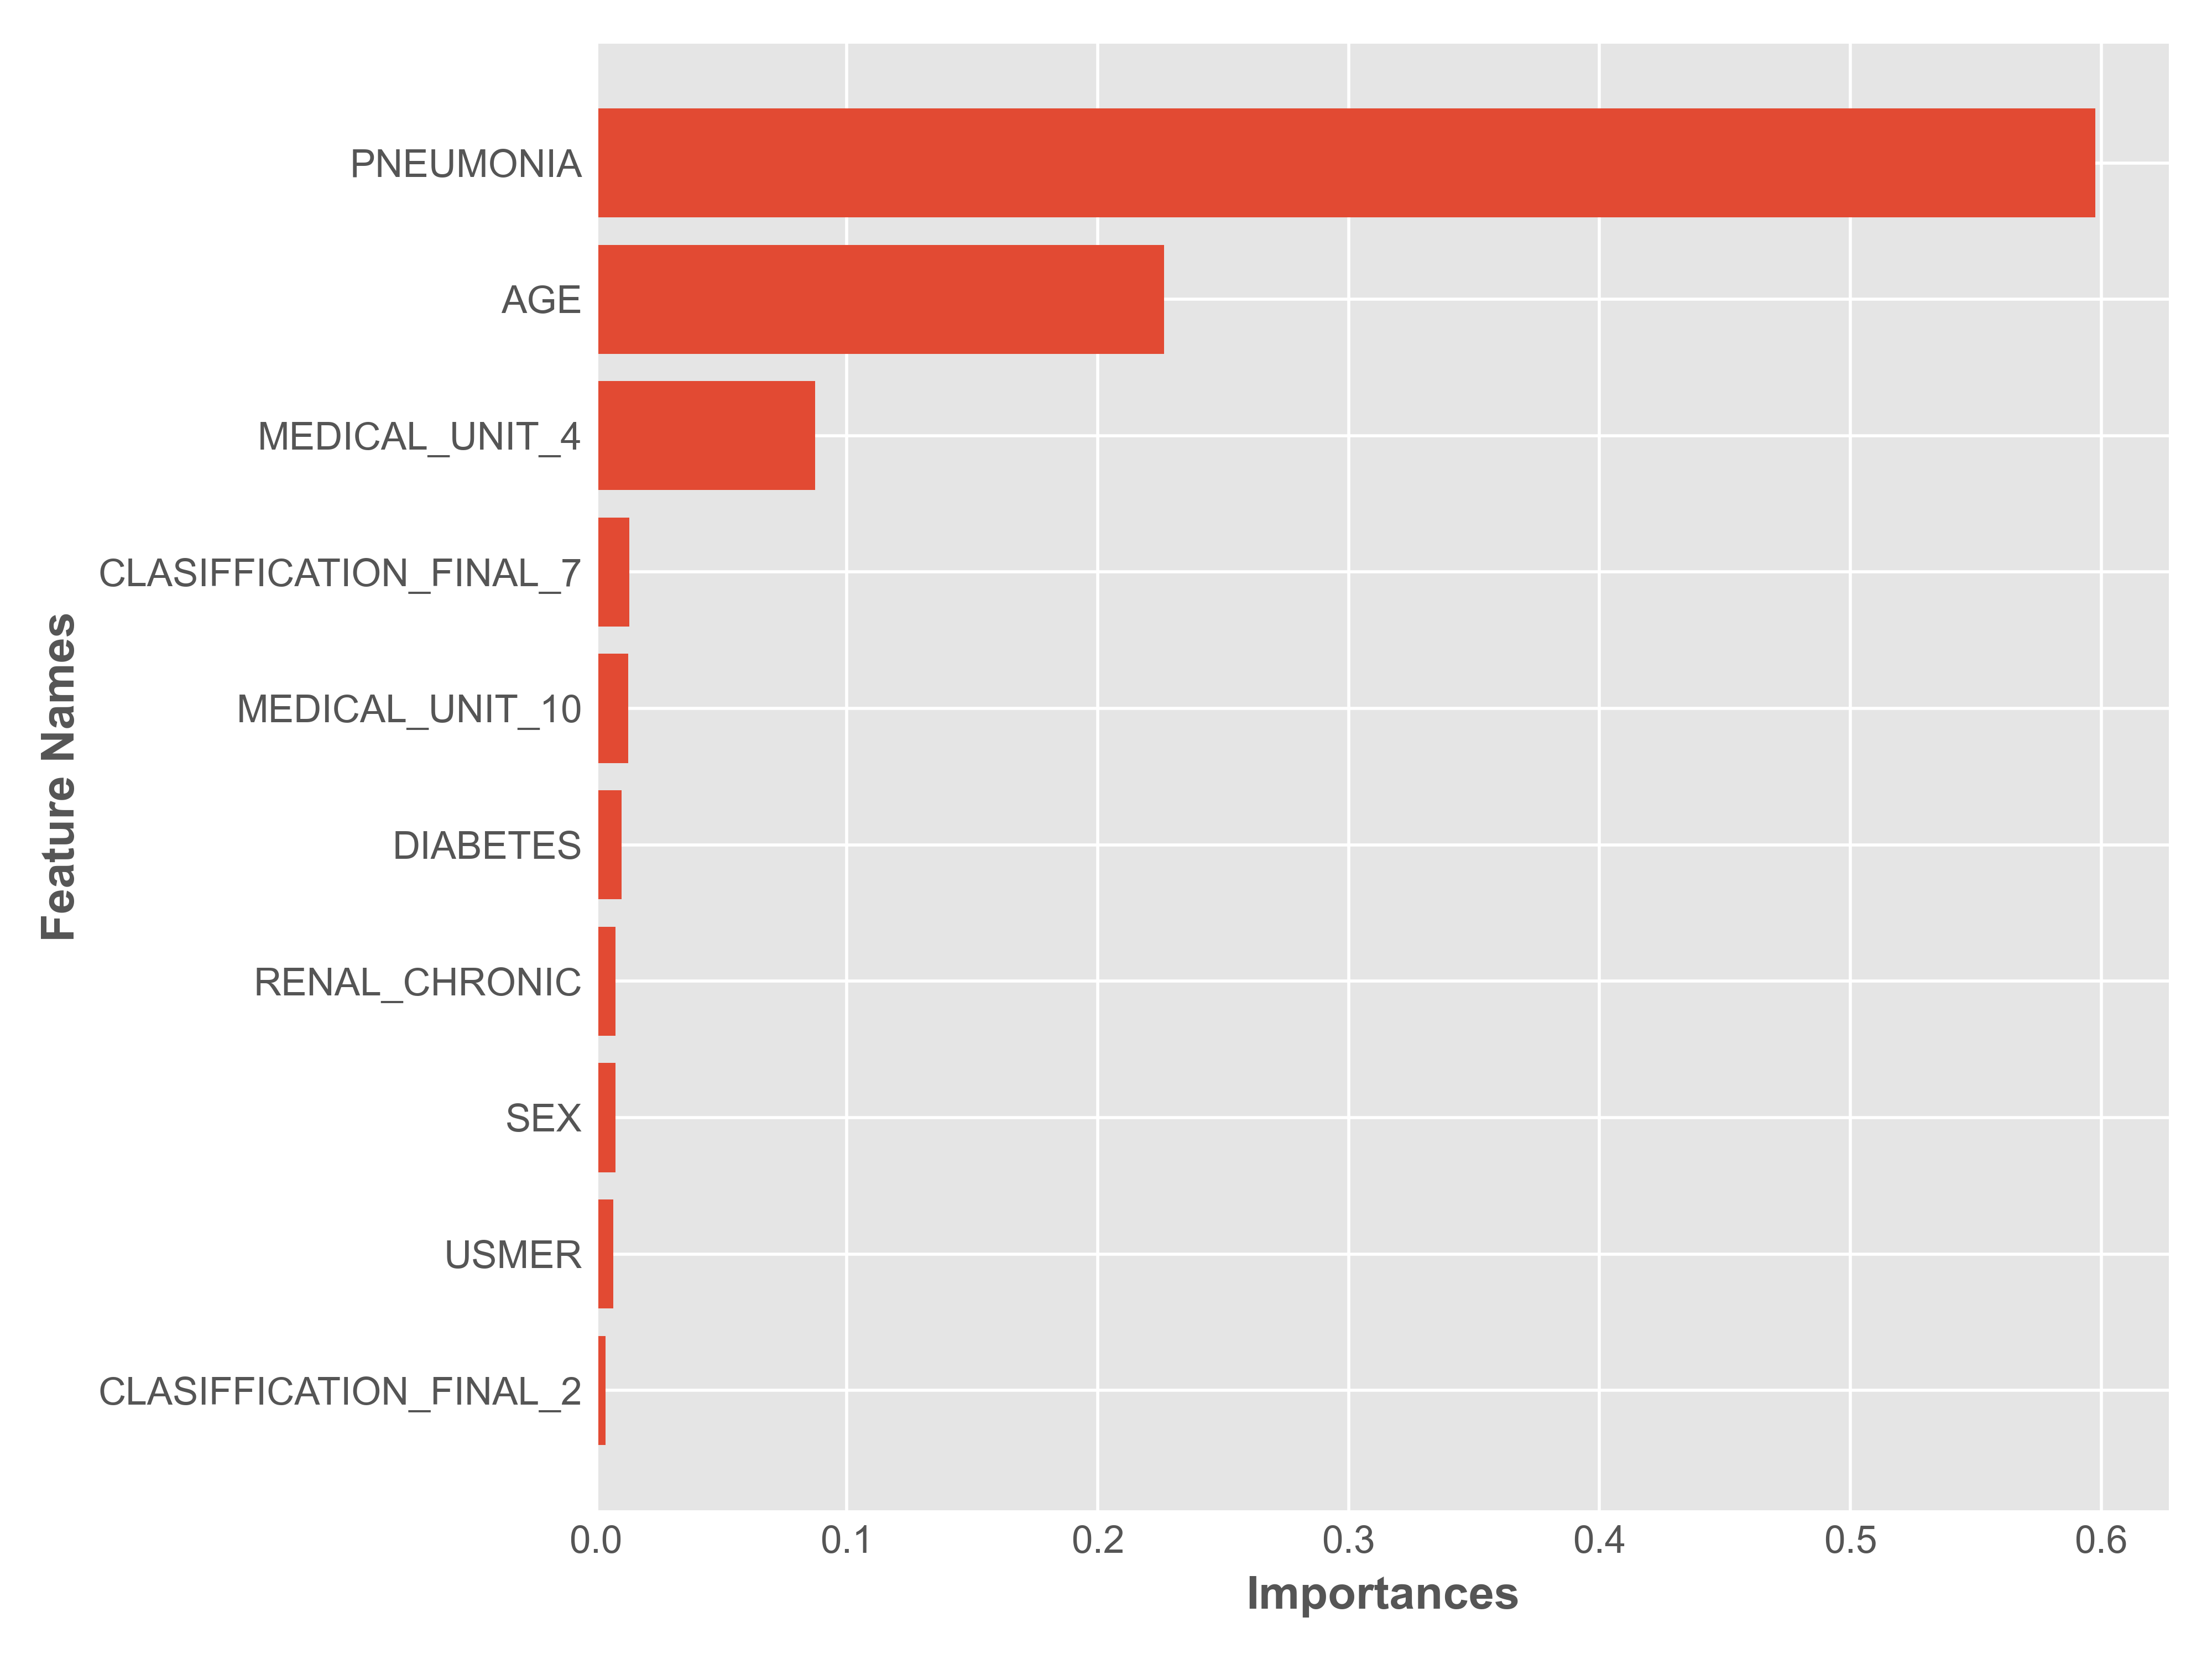
\includegraphics[width=0.6\linewidth]{pic/fefature_importance.png}
    \caption{Feature Importance Top10}
    \label{Feature Importance Top10}
\end{figure}


\section{Research Findings}

We will get the conclusion from both the algorithm and the model application scenario.

From an algorithmic perspective, this study compares five different algorithms and we conclude that using the decision tree model is most suitable for analyzing this dataset; the decision tree is highly explanatory and we can understand the algorithm's interpretation process from human decision logic; the decision tree makes predictions through a series of judgment rules that can be intuitively understood and interpreted. Each node of the decision tree represents a feature and the corresponding judgment condition, and the final leaf node represents the prediction result; the computational cost is really low compared with the other four algorithms according to practice; the correct rate of generalization performance can reach 88\%, and the accuracy rates of the training and validation sets are comparable, and there is no phenomenon of overfitting; in terms of stability, because the model has many parameters that can be adjusted, in fact, the selection of hyperparameters has a greater impact on the result;in terms of privacy protection, the decision tree usually does not involve direct manipulation of the original data during the training process, but constructs the tree structure by dividing the rules. This means that decision trees can protect the privacy of the original data to a certain extent.

From the results perspective, we measure the importance of features according to the way of feature importance of decision trees, i.e., Gini Importance: during the construction of decision trees, the importance of features is measured according to the splitting criterion (usually the Gini coefficient) of the features.Gini importance is calculated by considering, at each node, the number of splits of each feature and the weighting corresponding to that split The importance of a feature is evaluated by reducing the degree of impurity. higher Gini importance values indicate that the feature contributes more to the classification. We can conclude the following:

1.the presence or absence of pneumonia is crucial in the detection of the risk level of patients with COVID-19, if once a patient has pneumonia, his or her mortality rate will be greatly increased and he or she will be in a very dangerous state, therefore, if a patient is detected to have pneumonia, it means that he or she is probably already in a high-risk situation and needs to receive medical assistance in time; while if a patient is not yet detected to have pneumonia, it means that his or her symptoms of COVID-19 may be mild and does not need to receive If the patient has not yet been detected with pneumonia, the symptoms are probably mild and do not require much medical resources, but only need to ensure that they do not deteriorate further.

2.Patients with advanced age are more likely to be at high risk and more likely to die. For older patients, additional medical resources are needed because older patients generally have poorer immune systems than younger patients and require more medical attention and assistance. Patients of lower age may be able to recover with their own immune system without much medical resources.

3.The recovery of COVID-19 patients varies from one medical institution to another, probably due to the differences in medical services provided by medical centers in different regions. Therefore, it is recommended that the government should pay attention to medical resources and allocate resources equally to all medical centers, so that all people can receive equal medical resources fairly and should not have different high risk of illness due to the differences in medical resources.

\end{document}